\documentclass[fontset=fandol,aspectratio=169,11pt]{ctexbeamer}

\usetheme{Boadilla}
\usecolortheme{seahorse}
\setbeamertemplate{navigation symbols}{}
\setbeamertemplate{footline}[frame number]

\usepackage{booktabs}
\usepackage{tabularx}
\usepackage{array}
\usepackage{multirow}
\usepackage{pgfplots}
\usepackage{tikz}
\usetikzlibrary{positioning,arrows.meta,shapes.geometric}
\usepackage{xcolor}
\usepackage{hyperref}
\pgfplotsset{compat=1.18}

\AtBeginSubsection[]{
  \begin{frame}{\insertsection}
    \tableofcontents[currentsubsection, subsectionstyle=show/shaded/hide]
  \end{frame}
}

\definecolor{cmblue}{HTML}{1A5276}
\definecolor{cmgreen}{HTML}{1E8449}
\definecolor{cmorange}{HTML}{B9770E}
\definecolor{cmred}{HTML}{922B21}
\definecolor{cmgray}{HTML}{5C6773}

\setbeamercolor{title}{fg=cmblue}
\setbeamercolor{frametitle}{fg=cmblue}
\setbeamercolor{structure}{fg=cmblue}
\setbeamercolor{block title}{fg=white,bg=cmblue}
\setbeamercolor{block body}{fg=black,bg=blue!3}
\setbeamercolor{alerted text}{fg=cmred}

\newcommand{\code}[1]{\texttt{\detokenize{#1}}}
\newcommand{\metric}[1]{\texttt{#1}}
\newcommand{\tight}{\vspace{-0.35em}}

\title[Counting Manifolds 复现]{Chasing the Counting Manifold in Open LLMs\\—— 实验设计方案}
\subtitle{基于 Anthropic ``When Models Manipulate Manifolds'' 的开放模型复现}
\author{陈纳川}
\date{2026-06-11}

\begin{document}

% ============================================================
% 开场
% ============================================================
\begin{frame}
  \titlepage
\end{frame}

\begin{frame}{目录}
  \tableofcontents[hideallsubsections]
\end{frame}

% ============================================================
% Section 1: 背景与原文
% ============================================================
\section{背景与原论文}
\subsection{原论文核心主张}
% Original paper claims — Counting Manifold
% % Original paper claims — Counting Manifold
% % Original paper claims — Counting Manifold
% \input{01-background}

\begin{frame}{原论文：When Models Manipulate Manifolds}
\small
\begin{block}{Anthropic 的核心发现（2025）}
Anthropic 在 Claude 3.5 Haiku 中发现：语言模型的残差流中存在一个低维几何结构
——\textbf{计数流形（Counting Manifold）}——编码了 ``当前 token 距离上一个换行符的字符数'' 这一简单特征。
\end{block}

\begin{columns}[T,onlytextwidth]
\begin{column}{0.48\linewidth}
\textbf{三个核心主张：}
\begin{enumerate}
  \item \textbf{流形存在}：hidden state 中有一个低维（$\sim$6 维）子空间，其坐标与 chars-since-newline 高度对应
  \item \textbf{模型利用}：模型在预测换行符时会 ``读取'' 这个流形上的位置信息
  \item \textbf{SAE 可解释}：稀疏自编码器（SAE）的部分特征方向与该流形对齐，可定位 ``计数神经元''
\end{enumerate}
\end{column}
\begin{column}{0.48\linewidth}
\textbf{关键实验手段：}
\begin{itemize}
  \item 线性探针（Linear Probe）：hidden $\rightarrow$ char\_pos，测 R²
  \item PCA：对 mean hiddens 降维，可视化流形几何
  \item SAE：找到对 char\_pos 敏感的稀疏特征
  \item 干预实验：沿流形方向扰动 hidden state，观察换行预测变化
\end{itemize}
\end{column}
\end{columns}

\vspace{0.4em}
\begin{alertblock}{注意}
原论文使用 Claude 3.5 Haiku（闭源权重），其 SAE 和干预实验不可精确复现。
\end{alertblock}
\end{frame}

\begin{frame}{Counting Manifold 几何直觉}
\small
\begin{columns}[T,onlytextwidth]
\begin{column}{0.45\linewidth}
\textbf{chars\_since\_nl 的含义：}
\begin{itemize}
  \item 对每行文本按固定宽度（150 chars）自动换行
  \item 每个 token 标注：距离上一个 \code{\\n} 的字符偏移量
  \item 范围：$0 \sim 150$（0 = 行首，150 = 行尾）
\end{itemize}

\vspace{0.5em}
\textbf{流形的几何预期：}
\begin{itemize}
  \item PCA 前 2 个主成分应形成 \textbf{螺旋/环形} 结构
  \item 原因：char position 是循环变量（行首 $\approx$ 行尾，但偏移 1 不同）
  \item 更高维 PC 可能编码行内位置的非线性变化
\end{itemize}
\end{column}
\begin{column}{0.52\linewidth}
\begin{center}
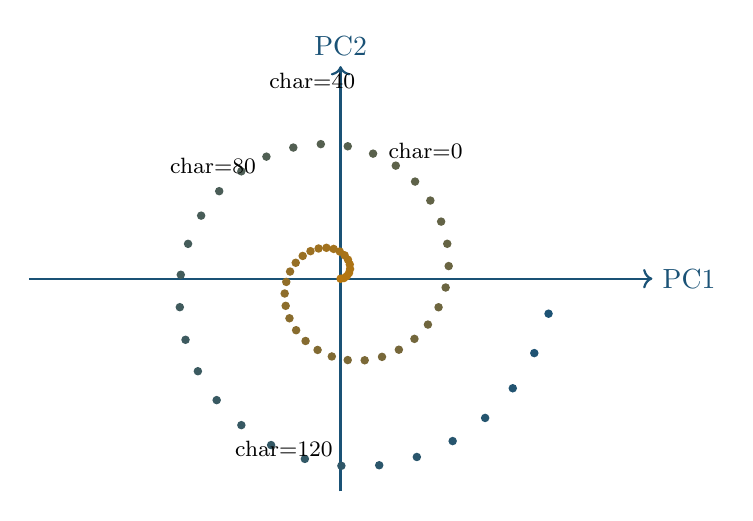
\begin{tikzpicture}[scale=1.8]
  % Spiral representing the counting manifold
  \draw[->, thick, cmblue] (-2.2, 0) -- (2.2, 0) node[right] {PC1};
  \draw[->, thick, cmblue] (0, -1.5) -- (0, 1.5) node[above] {PC2};
  % Draw spiral
  \foreach \t in {0, 0.2, 0.4, ..., 12.56} {
    \pgfmathsetmacro\r{\t * 0.12}
    \pgfmathsetmacro\x{\r * cos(\t r)}
    \pgfmathsetmacro\y{\r * sin(\t r)}
    \pgfmathsetmacro\c{int(100 * \t / 12.56)}
    \fill[cmblue!\c!cmorange] (\x, \y) circle (0.03);
  }
  \node[font=\footnotesize] at (0.6, 0.9) {char=0};
  \node[font=\footnotesize] at (-0.2, 1.4) {char=40};
  \node[font=\footnotesize] at (-0.9, 0.8) {char=80};
  \node[font=\footnotesize] at (-0.4, -1.2) {char=120};
\end{tikzpicture}
\end{center}
\vspace{-0.3em}
{\footnotesize 示意：PCA 投影后的螺旋结构\\每个点 = 某个 char position 的 mean hidden}
\end{column}
\end{columns}
\end{frame}


\begin{frame}{原论文：When Models Manipulate Manifolds}
\small
\begin{block}{Anthropic 的核心发现（2025）}
Anthropic 在 Claude 3.5 Haiku 中发现：语言模型的残差流中存在一个低维几何结构
——\textbf{计数流形（Counting Manifold）}——编码了 ``当前 token 距离上一个换行符的字符数'' 这一简单特征。
\end{block}

\begin{columns}[T,onlytextwidth]
\begin{column}{0.48\linewidth}
\textbf{三个核心主张：}
\begin{enumerate}
  \item \textbf{流形存在}：hidden state 中有一个低维（$\sim$6 维）子空间，其坐标与 chars-since-newline 高度对应
  \item \textbf{模型利用}：模型在预测换行符时会 ``读取'' 这个流形上的位置信息
  \item \textbf{SAE 可解释}：稀疏自编码器（SAE）的部分特征方向与该流形对齐，可定位 ``计数神经元''
\end{enumerate}
\end{column}
\begin{column}{0.48\linewidth}
\textbf{关键实验手段：}
\begin{itemize}
  \item 线性探针（Linear Probe）：hidden $\rightarrow$ char\_pos，测 R²
  \item PCA：对 mean hiddens 降维，可视化流形几何
  \item SAE：找到对 char\_pos 敏感的稀疏特征
  \item 干预实验：沿流形方向扰动 hidden state，观察换行预测变化
\end{itemize}
\end{column}
\end{columns}

\vspace{0.4em}
\begin{alertblock}{注意}
原论文使用 Claude 3.5 Haiku（闭源权重），其 SAE 和干预实验不可精确复现。
\end{alertblock}
\end{frame}

\begin{frame}{Counting Manifold 几何直觉}
\small
\begin{columns}[T,onlytextwidth]
\begin{column}{0.45\linewidth}
\textbf{chars\_since\_nl 的含义：}
\begin{itemize}
  \item 对每行文本按固定宽度（150 chars）自动换行
  \item 每个 token 标注：距离上一个 \code{\\n} 的字符偏移量
  \item 范围：$0 \sim 150$（0 = 行首，150 = 行尾）
\end{itemize}

\vspace{0.5em}
\textbf{流形的几何预期：}
\begin{itemize}
  \item PCA 前 2 个主成分应形成 \textbf{螺旋/环形} 结构
  \item 原因：char position 是循环变量（行首 $\approx$ 行尾，但偏移 1 不同）
  \item 更高维 PC 可能编码行内位置的非线性变化
\end{itemize}
\end{column}
\begin{column}{0.52\linewidth}
\begin{center}
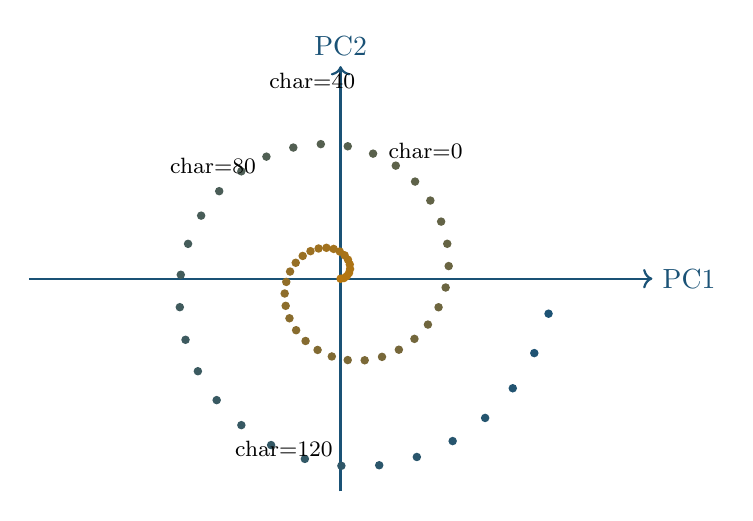
\begin{tikzpicture}[scale=1.8]
  % Spiral representing the counting manifold
  \draw[->, thick, cmblue] (-2.2, 0) -- (2.2, 0) node[right] {PC1};
  \draw[->, thick, cmblue] (0, -1.5) -- (0, 1.5) node[above] {PC2};
  % Draw spiral
  \foreach \t in {0, 0.2, 0.4, ..., 12.56} {
    \pgfmathsetmacro\r{\t * 0.12}
    \pgfmathsetmacro\x{\r * cos(\t r)}
    \pgfmathsetmacro\y{\r * sin(\t r)}
    \pgfmathsetmacro\c{int(100 * \t / 12.56)}
    \fill[cmblue!\c!cmorange] (\x, \y) circle (0.03);
  }
  \node[font=\footnotesize] at (0.6, 0.9) {char=0};
  \node[font=\footnotesize] at (-0.2, 1.4) {char=40};
  \node[font=\footnotesize] at (-0.9, 0.8) {char=80};
  \node[font=\footnotesize] at (-0.4, -1.2) {char=120};
\end{tikzpicture}
\end{center}
\vspace{-0.3em}
{\footnotesize 示意：PCA 投影后的螺旋结构\\每个点 = 某个 char position 的 mean hidden}
\end{column}
\end{columns}
\end{frame}


\begin{frame}{原论文：When Models Manipulate Manifolds}
\small
\begin{block}{Anthropic 的核心发现（2025）}
Anthropic 在 Claude 3.5 Haiku 中发现：语言模型的残差流中存在一个低维几何结构
——\textbf{计数流形（Counting Manifold）}——编码了 ``当前 token 距离上一个换行符的字符数'' 这一简单特征。
\end{block}

\begin{columns}[T,onlytextwidth]
\begin{column}{0.48\linewidth}
\textbf{三个核心主张：}
\begin{enumerate}
  \item \textbf{流形存在}：hidden state 中有一个低维（$\sim$6 维）子空间，其坐标与 chars-since-newline 高度对应
  \item \textbf{模型利用}：模型在预测换行符时会 ``读取'' 这个流形上的位置信息
  \item \textbf{SAE 可解释}：稀疏自编码器（SAE）的部分特征方向与该流形对齐，可定位 ``计数神经元''
\end{enumerate}
\end{column}
\begin{column}{0.48\linewidth}
\textbf{关键实验手段：}
\begin{itemize}
  \item 线性探针（Linear Probe）：hidden $\rightarrow$ char\_pos，测 R²
  \item PCA：对 mean hiddens 降维，可视化流形几何
  \item SAE：找到对 char\_pos 敏感的稀疏特征
  \item 干预实验：沿流形方向扰动 hidden state，观察换行预测变化
\end{itemize}
\end{column}
\end{columns}

\vspace{0.4em}
\begin{alertblock}{注意}
原论文使用 Claude 3.5 Haiku（闭源权重），其 SAE 和干预实验不可精确复现。
\end{alertblock}
\end{frame}

\begin{frame}{Counting Manifold 几何直觉}
\small
\begin{columns}[T,onlytextwidth]
\begin{column}{0.45\linewidth}
\textbf{chars\_since\_nl 的含义：}
\begin{itemize}
  \item 对每行文本按固定宽度（150 chars）自动换行
  \item 每个 token 标注：距离上一个 \code{\\n} 的字符偏移量
  \item 范围：$0 \sim 150$（0 = 行首，150 = 行尾）
\end{itemize}

\vspace{0.5em}
\textbf{流形的几何预期：}
\begin{itemize}
  \item PCA 前 2 个主成分应形成 \textbf{螺旋/环形} 结构
  \item 原因：char position 是循环变量（行首 $\approx$ 行尾，但偏移 1 不同）
  \item 更高维 PC 可能编码行内位置的非线性变化
\end{itemize}
\end{column}
\begin{column}{0.52\linewidth}
\begin{center}
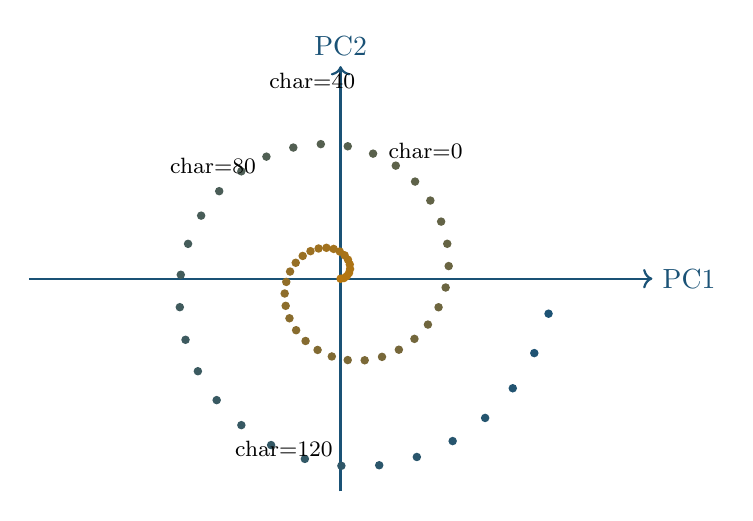
\begin{tikzpicture}[scale=1.8]
  % Spiral representing the counting manifold
  \draw[->, thick, cmblue] (-2.2, 0) -- (2.2, 0) node[right] {PC1};
  \draw[->, thick, cmblue] (0, -1.5) -- (0, 1.5) node[above] {PC2};
  % Draw spiral
  \foreach \t in {0, 0.2, 0.4, ..., 12.56} {
    \pgfmathsetmacro\r{\t * 0.12}
    \pgfmathsetmacro\x{\r * cos(\t r)}
    \pgfmathsetmacro\y{\r * sin(\t r)}
    \pgfmathsetmacro\c{int(100 * \t / 12.56)}
    \fill[cmblue!\c!cmorange] (\x, \y) circle (0.03);
  }
  \node[font=\footnotesize] at (0.6, 0.9) {char=0};
  \node[font=\footnotesize] at (-0.2, 1.4) {char=40};
  \node[font=\footnotesize] at (-0.9, 0.8) {char=80};
  \node[font=\footnotesize] at (-0.4, -1.2) {char=120};
\end{tikzpicture}
\end{center}
\vspace{-0.3em}
{\footnotesize 示意：PCA 投影后的螺旋结构\\每个点 = 某个 char position 的 mean hidden}
\end{column}
\end{columns}
\end{frame}

\subsection{本地复现范围}
% Reproduction scope
% % Reproduction scope
% % Reproduction scope
% \input{02-scope}

\begin{frame}{本地复现：能做什么、不能做什么}
\small
\begin{block}{复现基础}
本仓库 \code{corl-team/counting\_manifolds}（Apache 2.0）将 counting manifold 实验迁移到开放权重模型。
\end{block}

\begin{columns}[T,onlytextwidth]
\begin{column}{0.48\linewidth}
\textbf{能复现的：}
\begin{itemize}
  \item 完整 hidden state 收集（逐 token、逐层）
  \item chars\_since\_nl 线性探针（R², RMSE, MAE）
  \item mean hiddens PCA 降维与流形可视化
  \item GPT-2 SAE 特征激活分析 + PCA 投影
  \item 开放模型家族：Pythia、GPT-2、Gemma、Qwen3、Llama
\end{itemize}
\end{column}
\begin{column}{0.48\linewidth}
\textbf{不能复现的：}
\begin{itemize}
  \item Claude 3.5 Haiku 原始分析（无权重）
  \item Anthropic 内部的 SAE 训练与干预实验
  \item 原论文的 steering / intervention 验证
  \item Claude 特有的 feature 级别分析
\end{itemize}
\end{column}
\end{columns}

\vspace{0.4em}
\begin{block}{本次复现的两条路线}
\begin{tabularx}{\linewidth}{lllX}
\toprule
路线 & 模型 & 层数/维度 & 验证重点 \\
\midrule
\textbf{Pythia-70M} & EleutherAI/pythia-70m-deduped & 6 层 / 512-d & hidden state + probe + PCA 全流程 \\
\textbf{GPT-2} & openai-community/gpt2 & 12 层 / 768-d & 额外 SAE 特征提取 + PCA 投影 \\
\bottomrule
\end{tabularx}
\end{block}
\end{frame}

\begin{frame}{数据来源与处理}
\small
\begin{columns}[T,onlytextwidth]
\begin{column}{0.52\linewidth}
\textbf{数据集：HuggingFaceFW/fineweb}
\begin{itemize}
  \item train split，streaming 模式（不落地）
  \item 过滤：文本 $>$ 1500 chars（= 10 行 × 150），不含 \code{\\n}
  \item 取 1000 条，按 150 char 宽度自动换行
  \item Tokenizer：fast tokenizer + offset\_mapping 追踪字符位置
\end{itemize}

\vspace{0.4em}
\textbf{关键标注：chars\_since\_nl}
\begin{itemize}
  \item 对每个 token 计算：距上一个 \code{\\n} 的字符偏移
  \item 特殊 token / chat template token → 0
  \item 理论上限 = 150（line\_length）
\end{itemize}
\end{column}
\begin{column}{0.45\linewidth}
\textbf{处理管线：}
\begin{enumerate}
  \item \code{load\_dataset("fineweb", streaming=True)}
  \item \code{.filter()}：长度 + 无换行
  \item \code{islice(stream, 1000)} → materialize
  \item \code{wrap\_preserve\_newlines(width=150)}
  \item tokenize + offset\_mapping → chars\_since\_nl
  \item assert max(chars) $\le$ 150
\end{enumerate}
\end{column}
\end{columns}
\end{frame}


\begin{frame}{本地复现：能做什么、不能做什么}
\small
\begin{block}{复现基础}
本仓库 \code{corl-team/counting\_manifolds}（Apache 2.0）将 counting manifold 实验迁移到开放权重模型。
\end{block}

\begin{columns}[T,onlytextwidth]
\begin{column}{0.48\linewidth}
\textbf{能复现的：}
\begin{itemize}
  \item 完整 hidden state 收集（逐 token、逐层）
  \item chars\_since\_nl 线性探针（R², RMSE, MAE）
  \item mean hiddens PCA 降维与流形可视化
  \item GPT-2 SAE 特征激活分析 + PCA 投影
  \item 开放模型家族：Pythia、GPT-2、Gemma、Qwen3、Llama
\end{itemize}
\end{column}
\begin{column}{0.48\linewidth}
\textbf{不能复现的：}
\begin{itemize}
  \item Claude 3.5 Haiku 原始分析（无权重）
  \item Anthropic 内部的 SAE 训练与干预实验
  \item 原论文的 steering / intervention 验证
  \item Claude 特有的 feature 级别分析
\end{itemize}
\end{column}
\end{columns}

\vspace{0.4em}
\begin{block}{本次复现的两条路线}
\begin{tabularx}{\linewidth}{lllX}
\toprule
路线 & 模型 & 层数/维度 & 验证重点 \\
\midrule
\textbf{Pythia-70M} & EleutherAI/pythia-70m-deduped & 6 层 / 512-d & hidden state + probe + PCA 全流程 \\
\textbf{GPT-2} & openai-community/gpt2 & 12 层 / 768-d & 额外 SAE 特征提取 + PCA 投影 \\
\bottomrule
\end{tabularx}
\end{block}
\end{frame}

\begin{frame}{数据来源与处理}
\small
\begin{columns}[T,onlytextwidth]
\begin{column}{0.52\linewidth}
\textbf{数据集：HuggingFaceFW/fineweb}
\begin{itemize}
  \item train split，streaming 模式（不落地）
  \item 过滤：文本 $>$ 1500 chars（= 10 行 × 150），不含 \code{\\n}
  \item 取 1000 条，按 150 char 宽度自动换行
  \item Tokenizer：fast tokenizer + offset\_mapping 追踪字符位置
\end{itemize}

\vspace{0.4em}
\textbf{关键标注：chars\_since\_nl}
\begin{itemize}
  \item 对每个 token 计算：距上一个 \code{\\n} 的字符偏移
  \item 特殊 token / chat template token → 0
  \item 理论上限 = 150（line\_length）
\end{itemize}
\end{column}
\begin{column}{0.45\linewidth}
\textbf{处理管线：}
\begin{enumerate}
  \item \code{load\_dataset("fineweb", streaming=True)}
  \item \code{.filter()}：长度 + 无换行
  \item \code{islice(stream, 1000)} → materialize
  \item \code{wrap\_preserve\_newlines(width=150)}
  \item tokenize + offset\_mapping → chars\_since\_nl
  \item assert max(chars) $\le$ 150
\end{enumerate}
\end{column}
\end{columns}
\end{frame}


\begin{frame}{本地复现：能做什么、不能做什么}
\small
\begin{block}{复现基础}
本仓库 \code{corl-team/counting\_manifolds}（Apache 2.0）将 counting manifold 实验迁移到开放权重模型。
\end{block}

\begin{columns}[T,onlytextwidth]
\begin{column}{0.48\linewidth}
\textbf{能复现的：}
\begin{itemize}
  \item 完整 hidden state 收集（逐 token、逐层）
  \item chars\_since\_nl 线性探针（R², RMSE, MAE）
  \item mean hiddens PCA 降维与流形可视化
  \item GPT-2 SAE 特征激活分析 + PCA 投影
  \item 开放模型家族：Pythia、GPT-2、Gemma、Qwen3、Llama
\end{itemize}
\end{column}
\begin{column}{0.48\linewidth}
\textbf{不能复现的：}
\begin{itemize}
  \item Claude 3.5 Haiku 原始分析（无权重）
  \item Anthropic 内部的 SAE 训练与干预实验
  \item 原论文的 steering / intervention 验证
  \item Claude 特有的 feature 级别分析
\end{itemize}
\end{column}
\end{columns}

\vspace{0.4em}
\begin{block}{本次复现的两条路线}
\begin{tabularx}{\linewidth}{lllX}
\toprule
路线 & 模型 & 层数/维度 & 验证重点 \\
\midrule
\textbf{Pythia-70M} & EleutherAI/pythia-70m-deduped & 6 层 / 512-d & hidden state + probe + PCA 全流程 \\
\textbf{GPT-2} & openai-community/gpt2 & 12 层 / 768-d & 额外 SAE 特征提取 + PCA 投影 \\
\bottomrule
\end{tabularx}
\end{block}
\end{frame}

\begin{frame}{数据来源与处理}
\small
\begin{columns}[T,onlytextwidth]
\begin{column}{0.52\linewidth}
\textbf{数据集：HuggingFaceFW/fineweb}
\begin{itemize}
  \item train split，streaming 模式（不落地）
  \item 过滤：文本 $>$ 1500 chars（= 10 行 × 150），不含 \code{\\n}
  \item 取 1000 条，按 150 char 宽度自动换行
  \item Tokenizer：fast tokenizer + offset\_mapping 追踪字符位置
\end{itemize}

\vspace{0.4em}
\textbf{关键标注：chars\_since\_nl}
\begin{itemize}
  \item 对每个 token 计算：距上一个 \code{\\n} 的字符偏移
  \item 特殊 token / chat template token → 0
  \item 理论上限 = 150（line\_length）
\end{itemize}
\end{column}
\begin{column}{0.45\linewidth}
\textbf{处理管线：}
\begin{enumerate}
  \item \code{load\_dataset("fineweb", streaming=True)}
  \item \code{.filter()}：长度 + 无换行
  \item \code{islice(stream, 1000)} → materialize
  \item \code{wrap\_preserve\_newlines(width=150)}
  \item tokenize + offset\_mapping → chars\_since\_nl
  \item assert max(chars) $\le$ 150
\end{enumerate}
\end{column}
\end{columns}
\end{frame}


% ============================================================
% Section 2: 实验管线
% ============================================================
\section{实验管线}
\subsection{数据流总览}
% Pipeline overview
% % Pipeline overview
% % Pipeline overview
% \input{03-pipeline}

\begin{frame}{实验管线总览}
\footnotesize
\begin{tabularx}{\linewidth}{cXl}
\toprule
步骤 & 流程 & 产物 \\
\midrule
\textbf{1. 数据准备} & FineWeb → 过滤 → 换行包装 → tokenize + chars\_since\_nl 标注 & 1000 条 tokenized 样本 \\
\textbf{2. LM 评估} & 前向传播 → next-token NLL loss / accuracy / newline prob & \code{lm\_metrics.csv}, \code{newline\_probs.npy} \\
\textbf{3. 逐层分析} & 每层：collect hiddens → mean by char count → linear probe → PCA & \code{metrics.csv}, \code{mean\_hiddens.npy} \\
\textbf{4. SAE 分析} & (GPT-2 only) SAE encode → per-count activation → top features → PCA 投影 & \code{sae\_mean\_acts.npy}, \code{top\_sae\_features\_projected.npy} \\
\bottomrule
\end{tabularx}

\vspace{0.6em}
\begin{center}
\begin{tikzpicture}[
  node distance=2.8cm,
  box/.style={draw, rounded corners=3pt, align=center, minimum width=3.2cm, minimum height=1.0cm, font=\footnotesize},
  arr/.style={->, thick, color=cmblue}
]
\node[box, fill=cmblue!10] (data) {FineWeb\\原始文本};
\node[box, fill=cmblue!10, right=of data] (tok) {Tokenization\\+ chars\_since\_nl};
\node[box, fill=cmgreen!10, right=of tok] (lm) {LM 评估\\loss/acc/newline};
\node[box, fill=cmorange!10, below=of tok] (layer) {逐层分析\\probe + PCA};
\node[box, fill=cmred!10, below=of lm] (sae) {SAE 分析\\(仅 GPT-2)};
\draw[arr] (data) -- (tok);
\draw[arr] (tok) -- (lm);
\draw[arr] (tok) -- (layer);
\draw[arr] (layer) -- (sae);
\end{tikzpicture}
\end{center}
\end{frame}

\begin{frame}{步骤 1：LM 评估——模型基础能力基线}
\small
\begin{block}{评估内容}
在 1000 条 FineWeb 样本上做一次完整前向传播，计算 next-token 预测指标。
\end{block}

\begin{tabularx}{\linewidth}{l>{\raggedright\arraybackslash}p{5cm}l}
\toprule
指标 & 含义 & 方向 \\
\midrule
\metric{lm\_loss} & next-token NLL loss（仅 valid tokens） & $\downarrow$ \\
\metric{lm\_acc} & next-token argmax 准确率 & $\uparrow$ \\
\metric{lm\_acc\_if\_newline} & 当 gold token 含 \code{\\n} 时，精确命中准确率 & $\uparrow$ \\
\metric{lm\_acc\_if\_newline\_any} & 当 gold token 含 \code{\\n} 时，预测任一含 \code{\\n} token 的准确率 & $\uparrow$ \\
\metric{mean\_prob\_if\_newline} & gold token 含 \code{\\n} 时，所有含 \code{\\n} token 的概率质量均值 & $\uparrow$ \\
\bottomrule
\end{tabularx}

\vspace{0.4em}
\begin{itemize}
  \item 如果 LM 指标极差（如 loss 异常高），说明模型加载或数据 pipeline 有问题
  \item newline 相关指标反映模型对换行位置的敏感度，为后续 counting manifold 提供行为基线
\end{itemize}
\end{frame}


\begin{frame}{实验管线总览}
\footnotesize
\begin{tabularx}{\linewidth}{cXl}
\toprule
步骤 & 流程 & 产物 \\
\midrule
\textbf{1. 数据准备} & FineWeb → 过滤 → 换行包装 → tokenize + chars\_since\_nl 标注 & 1000 条 tokenized 样本 \\
\textbf{2. LM 评估} & 前向传播 → next-token NLL loss / accuracy / newline prob & \code{lm\_metrics.csv}, \code{newline\_probs.npy} \\
\textbf{3. 逐层分析} & 每层：collect hiddens → mean by char count → linear probe → PCA & \code{metrics.csv}, \code{mean\_hiddens.npy} \\
\textbf{4. SAE 分析} & (GPT-2 only) SAE encode → per-count activation → top features → PCA 投影 & \code{sae\_mean\_acts.npy}, \code{top\_sae\_features\_projected.npy} \\
\bottomrule
\end{tabularx}

\vspace{0.6em}
\begin{center}
\begin{tikzpicture}[
  node distance=2.8cm,
  box/.style={draw, rounded corners=3pt, align=center, minimum width=3.2cm, minimum height=1.0cm, font=\footnotesize},
  arr/.style={->, thick, color=cmblue}
]
\node[box, fill=cmblue!10] (data) {FineWeb\\原始文本};
\node[box, fill=cmblue!10, right=of data] (tok) {Tokenization\\+ chars\_since\_nl};
\node[box, fill=cmgreen!10, right=of tok] (lm) {LM 评估\\loss/acc/newline};
\node[box, fill=cmorange!10, below=of tok] (layer) {逐层分析\\probe + PCA};
\node[box, fill=cmred!10, below=of lm] (sae) {SAE 分析\\(仅 GPT-2)};
\draw[arr] (data) -- (tok);
\draw[arr] (tok) -- (lm);
\draw[arr] (tok) -- (layer);
\draw[arr] (layer) -- (sae);
\end{tikzpicture}
\end{center}
\end{frame}

\begin{frame}{步骤 1：LM 评估——模型基础能力基线}
\small
\begin{block}{评估内容}
在 1000 条 FineWeb 样本上做一次完整前向传播，计算 next-token 预测指标。
\end{block}

\begin{tabularx}{\linewidth}{l>{\raggedright\arraybackslash}p{5cm}l}
\toprule
指标 & 含义 & 方向 \\
\midrule
\metric{lm\_loss} & next-token NLL loss（仅 valid tokens） & $\downarrow$ \\
\metric{lm\_acc} & next-token argmax 准确率 & $\uparrow$ \\
\metric{lm\_acc\_if\_newline} & 当 gold token 含 \code{\\n} 时，精确命中准确率 & $\uparrow$ \\
\metric{lm\_acc\_if\_newline\_any} & 当 gold token 含 \code{\\n} 时，预测任一含 \code{\\n} token 的准确率 & $\uparrow$ \\
\metric{mean\_prob\_if\_newline} & gold token 含 \code{\\n} 时，所有含 \code{\\n} token 的概率质量均值 & $\uparrow$ \\
\bottomrule
\end{tabularx}

\vspace{0.4em}
\begin{itemize}
  \item 如果 LM 指标极差（如 loss 异常高），说明模型加载或数据 pipeline 有问题
  \item newline 相关指标反映模型对换行位置的敏感度，为后续 counting manifold 提供行为基线
\end{itemize}
\end{frame}


\begin{frame}{实验管线总览}
\footnotesize
\begin{tabularx}{\linewidth}{cXl}
\toprule
步骤 & 流程 & 产物 \\
\midrule
\textbf{1. 数据准备} & FineWeb → 过滤 → 换行包装 → tokenize + chars\_since\_nl 标注 & 1000 条 tokenized 样本 \\
\textbf{2. LM 评估} & 前向传播 → next-token NLL loss / accuracy / newline prob & \code{lm\_metrics.csv}, \code{newline\_probs.npy} \\
\textbf{3. 逐层分析} & 每层：collect hiddens → mean by char count → linear probe → PCA & \code{metrics.csv}, \code{mean\_hiddens.npy} \\
\textbf{4. SAE 分析} & (GPT-2 only) SAE encode → per-count activation → top features → PCA 投影 & \code{sae\_mean\_acts.npy}, \code{top\_sae\_features\_projected.npy} \\
\bottomrule
\end{tabularx}

\vspace{0.6em}
\begin{center}
\begin{tikzpicture}[
  node distance=2.8cm,
  box/.style={draw, rounded corners=3pt, align=center, minimum width=3.2cm, minimum height=1.0cm, font=\footnotesize},
  arr/.style={->, thick, color=cmblue}
]
\node[box, fill=cmblue!10] (data) {FineWeb\\原始文本};
\node[box, fill=cmblue!10, right=of data] (tok) {Tokenization\\+ chars\_since\_nl};
\node[box, fill=cmgreen!10, right=of tok] (lm) {LM 评估\\loss/acc/newline};
\node[box, fill=cmorange!10, below=of tok] (layer) {逐层分析\\probe + PCA};
\node[box, fill=cmred!10, below=of lm] (sae) {SAE 分析\\(仅 GPT-2)};
\draw[arr] (data) -- (tok);
\draw[arr] (tok) -- (lm);
\draw[arr] (tok) -- (layer);
\draw[arr] (layer) -- (sae);
\end{tikzpicture}
\end{center}
\end{frame}

\begin{frame}{步骤 1：LM 评估——模型基础能力基线}
\small
\begin{block}{评估内容}
在 1000 条 FineWeb 样本上做一次完整前向传播，计算 next-token 预测指标。
\end{block}

\begin{tabularx}{\linewidth}{l>{\raggedright\arraybackslash}p{5cm}l}
\toprule
指标 & 含义 & 方向 \\
\midrule
\metric{lm\_loss} & next-token NLL loss（仅 valid tokens） & $\downarrow$ \\
\metric{lm\_acc} & next-token argmax 准确率 & $\uparrow$ \\
\metric{lm\_acc\_if\_newline} & 当 gold token 含 \code{\\n} 时，精确命中准确率 & $\uparrow$ \\
\metric{lm\_acc\_if\_newline\_any} & 当 gold token 含 \code{\\n} 时，预测任一含 \code{\\n} token 的准确率 & $\uparrow$ \\
\metric{mean\_prob\_if\_newline} & gold token 含 \code{\\n} 时，所有含 \code{\\n} token 的概率质量均值 & $\uparrow$ \\
\bottomrule
\end{tabularx}

\vspace{0.4em}
\begin{itemize}
  \item 如果 LM 指标极差（如 loss 异常高），说明模型加载或数据 pipeline 有问题
  \item newline 相关指标反映模型对换行位置的敏感度，为后续 counting manifold 提供行为基线
\end{itemize}
\end{frame}

\subsection{分析方法详解}
% Analysis methods
% % Analysis methods
% % Analysis methods
% \input{04-methods}

\begin{frame}{步骤 2：逐层 Hidden State 收集}
\small
\begin{columns}[T,onlytextwidth]
\begin{column}{0.55\linewidth}
\textbf{collect\_layer\_hiddens()：}
\begin{enumerate}
  \item 逐 batch 前向传播，\code{output\_hidden\_states=True}
  \item 取出目标层的 hidden state：\code{hs[layer\_idx+1]}
  \item 按 unpadded length 截取，返回 \code{List[[T, H]]}
  \item 全部存在 CPU 内存（detach + cpu）
\end{enumerate}
\end{column}
\begin{column}{0.42\linewidth}
\textbf{mean\_hidden\_by\_chars\_since\_nl()：}
\begin{enumerate}
  \item 对每个 char count $c \in [0, 150]$
  \item 收集所有 chars\_since\_nl $= c$ 的 hidden state
  \item 取均值 → \code{[151, H]} 矩阵
  \item 每行 = 该 char position 的 ``原型向量''
\end{enumerate}
\end{column}
\end{columns}

\vspace{0.4em}
\begin{block}{为什么用 mean hidden？}
单个 token 的 hidden state 噪声很大（受上下文、语义等影响）。按 char count 分组求均值后，
消去了语义噪声，保留纯粹的 position 信号。这个 \textbf{151 × H 的均值矩阵}就是 counting manifold 的载体。
\end{block}
\end{frame}

\begin{frame}{步骤 2：线性探针（Linear Probe）}
\small
\begin{block}{方法}
对所有 token 的 hidden state $X \in \mathbb{R}^{N \times H}$ 和对应的 chars\_since\_nl $y \in \mathbb{R}^N$，
拟合最小二乘回归：$\hat{y} = Xw + b$。
\end{block}

\begin{columns}[T,onlytextwidth]
\begin{column}{0.48\linewidth}
\textbf{指标：}
\begin{itemize}
  \item \textbf{R²}：hidden state 线性可解释的 char position 方差比例（主指标）
  \item \textbf{RMSE}：预测的均方根误差（chars），随机基线 $\approx 43$
  \item \textbf{MAE}：平均绝对误差
\end{itemize}
\end{column}
\begin{column}{0.48\linewidth}
\textbf{解读：}
\begin{itemize}
  \item R² $>$ 0.5 → counting 信息以线性可读方式存在
  \item R² $\approx$ 0 → 该层不编码 position
  \item R² 的最高层通常出现在中间层（非最后层）
\end{itemize}
\end{column}
\end{columns}

\vspace{0.4em}
\begin{block}{局限性}
线性探针只能检测\textbf{线性可分离}的信息。如果 char position 以非线性方式编码，R² 会低估信息量。
PCA 部分互补了这一局限。
\end{block}
\end{frame}

\begin{frame}{步骤 3：PCA 流形可视化}
\small
\begin{columns}[T,onlytextwidth]
\begin{column}{0.52\linewidth}
\textbf{pca\_per\_layer()：}
\begin{enumerate}
  \item 输入：mean hiddens \code{[151, H]}
  \item 省略前 \code{n\_omit=20} 个 char counts（行首噪声大）
  \item 对剩余 \code{[131, H]} 做 PCA（full SVD）
  \item 取前 \code{n\_components=6} 个主成分
  \item 返回：投影坐标 \code{[151, 6]} + explained variance ratio
\end{enumerate}
\end{column}
\begin{column}{0.45\linewidth}
\textbf{关键观察：}
\begin{itemize}
  \item PC1-PC2 是否呈螺旋/环形？
  \item 前 6 PC 解释了多少方差？（$>$50\% = 强低维结构）
  \item 各层的流形形状如何变化？
  \item SAE features 投影到 PCA 空间后的方向？
\end{itemize}
\end{column}
\end{columns}

\vspace{0.4em}
\begin{block}{为什么省略前 20 个 counts？}
行首位置（char 0--19）的 hidden state 可能受 BOS token、首词效应等混杂，去掉后 PCA 更干净地捕获纯 position 信号。
\end{block}
\end{frame}

\begin{frame}{步骤 4：SAE 特征分析（仅 GPT-2）}
\small
\begin{block}{SAE 接入}
GPT-2 使用 Joseph Bloom 的 \code{gpt2-small-resid-post-v5-128k} SAE（128k features/layer）。
通过 \code{sae\_lens} 库加载，逐 char count 计算 feature activations。
\end{block}

\begin{columns}[T,onlytextwidth]
\begin{column}{0.50\linewidth}
\textbf{分析流程：}
\begin{enumerate}
  \item \code{sae.encode(hidden)} → sparse activations
  \item 乘以 \code{W\_dec} norm（还原真实激活幅度）
  \item 逐 char count 取均值 → \code{[150, 128k]}
  \item 按 std 排序，取 top 100 features
  \item 将 top feature 的 W\_dec 方向投影到 PCA 空间
\end{enumerate}
\end{column}
\begin{column}{0.47\linewidth}
\textbf{核心问题：}
\begin{itemize}
  \item SAE top features 是否沿 counting manifold 方向排列？
  \item 是否存在 ``计数神经元''（激活随 position 单调/周期变化）？
  \item SAE 特征方向的 PCA 投影是否形成有意义的几何结构？
\end{itemize}
\end{column}
\end{columns}

\vspace{0.4em}
\textbf{产物：}
\code{sae\_mean\_acts.npy}（[L, 150, 128k]）、\code{top\_sae\_features\_projected.npy}（[L, 100, 6]）、\code{mean\_hiddens\_pca\_sae\_spanned\_*.npy}
\end{frame}


\begin{frame}{步骤 2：逐层 Hidden State 收集}
\small
\begin{columns}[T,onlytextwidth]
\begin{column}{0.55\linewidth}
\textbf{collect\_layer\_hiddens()：}
\begin{enumerate}
  \item 逐 batch 前向传播，\code{output\_hidden\_states=True}
  \item 取出目标层的 hidden state：\code{hs[layer\_idx+1]}
  \item 按 unpadded length 截取，返回 \code{List[[T, H]]}
  \item 全部存在 CPU 内存（detach + cpu）
\end{enumerate}
\end{column}
\begin{column}{0.42\linewidth}
\textbf{mean\_hidden\_by\_chars\_since\_nl()：}
\begin{enumerate}
  \item 对每个 char count $c \in [0, 150]$
  \item 收集所有 chars\_since\_nl $= c$ 的 hidden state
  \item 取均值 → \code{[151, H]} 矩阵
  \item 每行 = 该 char position 的 ``原型向量''
\end{enumerate}
\end{column}
\end{columns}

\vspace{0.4em}
\begin{block}{为什么用 mean hidden？}
单个 token 的 hidden state 噪声很大（受上下文、语义等影响）。按 char count 分组求均值后，
消去了语义噪声，保留纯粹的 position 信号。这个 \textbf{151 × H 的均值矩阵}就是 counting manifold 的载体。
\end{block}
\end{frame}

\begin{frame}{步骤 2：线性探针（Linear Probe）}
\small
\begin{block}{方法}
对所有 token 的 hidden state $X \in \mathbb{R}^{N \times H}$ 和对应的 chars\_since\_nl $y \in \mathbb{R}^N$，
拟合最小二乘回归：$\hat{y} = Xw + b$。
\end{block}

\begin{columns}[T,onlytextwidth]
\begin{column}{0.48\linewidth}
\textbf{指标：}
\begin{itemize}
  \item \textbf{R²}：hidden state 线性可解释的 char position 方差比例（主指标）
  \item \textbf{RMSE}：预测的均方根误差（chars），随机基线 $\approx 43$
  \item \textbf{MAE}：平均绝对误差
\end{itemize}
\end{column}
\begin{column}{0.48\linewidth}
\textbf{解读：}
\begin{itemize}
  \item R² $>$ 0.5 → counting 信息以线性可读方式存在
  \item R² $\approx$ 0 → 该层不编码 position
  \item R² 的最高层通常出现在中间层（非最后层）
\end{itemize}
\end{column}
\end{columns}

\vspace{0.4em}
\begin{block}{局限性}
线性探针只能检测\textbf{线性可分离}的信息。如果 char position 以非线性方式编码，R² 会低估信息量。
PCA 部分互补了这一局限。
\end{block}
\end{frame}

\begin{frame}{步骤 3：PCA 流形可视化}
\small
\begin{columns}[T,onlytextwidth]
\begin{column}{0.52\linewidth}
\textbf{pca\_per\_layer()：}
\begin{enumerate}
  \item 输入：mean hiddens \code{[151, H]}
  \item 省略前 \code{n\_omit=20} 个 char counts（行首噪声大）
  \item 对剩余 \code{[131, H]} 做 PCA（full SVD）
  \item 取前 \code{n\_components=6} 个主成分
  \item 返回：投影坐标 \code{[151, 6]} + explained variance ratio
\end{enumerate}
\end{column}
\begin{column}{0.45\linewidth}
\textbf{关键观察：}
\begin{itemize}
  \item PC1-PC2 是否呈螺旋/环形？
  \item 前 6 PC 解释了多少方差？（$>$50\% = 强低维结构）
  \item 各层的流形形状如何变化？
  \item SAE features 投影到 PCA 空间后的方向？
\end{itemize}
\end{column}
\end{columns}

\vspace{0.4em}
\begin{block}{为什么省略前 20 个 counts？}
行首位置（char 0--19）的 hidden state 可能受 BOS token、首词效应等混杂，去掉后 PCA 更干净地捕获纯 position 信号。
\end{block}
\end{frame}

\begin{frame}{步骤 4：SAE 特征分析（仅 GPT-2）}
\small
\begin{block}{SAE 接入}
GPT-2 使用 Joseph Bloom 的 \code{gpt2-small-resid-post-v5-128k} SAE（128k features/layer）。
通过 \code{sae\_lens} 库加载，逐 char count 计算 feature activations。
\end{block}

\begin{columns}[T,onlytextwidth]
\begin{column}{0.50\linewidth}
\textbf{分析流程：}
\begin{enumerate}
  \item \code{sae.encode(hidden)} → sparse activations
  \item 乘以 \code{W\_dec} norm（还原真实激活幅度）
  \item 逐 char count 取均值 → \code{[150, 128k]}
  \item 按 std 排序，取 top 100 features
  \item 将 top feature 的 W\_dec 方向投影到 PCA 空间
\end{enumerate}
\end{column}
\begin{column}{0.47\linewidth}
\textbf{核心问题：}
\begin{itemize}
  \item SAE top features 是否沿 counting manifold 方向排列？
  \item 是否存在 ``计数神经元''（激活随 position 单调/周期变化）？
  \item SAE 特征方向的 PCA 投影是否形成有意义的几何结构？
\end{itemize}
\end{column}
\end{columns}

\vspace{0.4em}
\textbf{产物：}
\code{sae\_mean\_acts.npy}（[L, 150, 128k]）、\code{top\_sae\_features\_projected.npy}（[L, 100, 6]）、\code{mean\_hiddens\_pca\_sae\_spanned\_*.npy}
\end{frame}


\begin{frame}{步骤 2：逐层 Hidden State 收集}
\small
\begin{columns}[T,onlytextwidth]
\begin{column}{0.55\linewidth}
\textbf{collect\_layer\_hiddens()：}
\begin{enumerate}
  \item 逐 batch 前向传播，\code{output\_hidden\_states=True}
  \item 取出目标层的 hidden state：\code{hs[layer\_idx+1]}
  \item 按 unpadded length 截取，返回 \code{List[[T, H]]}
  \item 全部存在 CPU 内存（detach + cpu）
\end{enumerate}
\end{column}
\begin{column}{0.42\linewidth}
\textbf{mean\_hidden\_by\_chars\_since\_nl()：}
\begin{enumerate}
  \item 对每个 char count $c \in [0, 150]$
  \item 收集所有 chars\_since\_nl $= c$ 的 hidden state
  \item 取均值 → \code{[151, H]} 矩阵
  \item 每行 = 该 char position 的 ``原型向量''
\end{enumerate}
\end{column}
\end{columns}

\vspace{0.4em}
\begin{block}{为什么用 mean hidden？}
单个 token 的 hidden state 噪声很大（受上下文、语义等影响）。按 char count 分组求均值后，
消去了语义噪声，保留纯粹的 position 信号。这个 \textbf{151 × H 的均值矩阵}就是 counting manifold 的载体。
\end{block}
\end{frame}

\begin{frame}{步骤 2：线性探针（Linear Probe）}
\small
\begin{block}{方法}
对所有 token 的 hidden state $X \in \mathbb{R}^{N \times H}$ 和对应的 chars\_since\_nl $y \in \mathbb{R}^N$，
拟合最小二乘回归：$\hat{y} = Xw + b$。
\end{block}

\begin{columns}[T,onlytextwidth]
\begin{column}{0.48\linewidth}
\textbf{指标：}
\begin{itemize}
  \item \textbf{R²}：hidden state 线性可解释的 char position 方差比例（主指标）
  \item \textbf{RMSE}：预测的均方根误差（chars），随机基线 $\approx 43$
  \item \textbf{MAE}：平均绝对误差
\end{itemize}
\end{column}
\begin{column}{0.48\linewidth}
\textbf{解读：}
\begin{itemize}
  \item R² $>$ 0.5 → counting 信息以线性可读方式存在
  \item R² $\approx$ 0 → 该层不编码 position
  \item R² 的最高层通常出现在中间层（非最后层）
\end{itemize}
\end{column}
\end{columns}

\vspace{0.4em}
\begin{block}{局限性}
线性探针只能检测\textbf{线性可分离}的信息。如果 char position 以非线性方式编码，R² 会低估信息量。
PCA 部分互补了这一局限。
\end{block}
\end{frame}

\begin{frame}{步骤 3：PCA 流形可视化}
\small
\begin{columns}[T,onlytextwidth]
\begin{column}{0.52\linewidth}
\textbf{pca\_per\_layer()：}
\begin{enumerate}
  \item 输入：mean hiddens \code{[151, H]}
  \item 省略前 \code{n\_omit=20} 个 char counts（行首噪声大）
  \item 对剩余 \code{[131, H]} 做 PCA（full SVD）
  \item 取前 \code{n\_components=6} 个主成分
  \item 返回：投影坐标 \code{[151, 6]} + explained variance ratio
\end{enumerate}
\end{column}
\begin{column}{0.45\linewidth}
\textbf{关键观察：}
\begin{itemize}
  \item PC1-PC2 是否呈螺旋/环形？
  \item 前 6 PC 解释了多少方差？（$>$50\% = 强低维结构）
  \item 各层的流形形状如何变化？
  \item SAE features 投影到 PCA 空间后的方向？
\end{itemize}
\end{column}
\end{columns}

\vspace{0.4em}
\begin{block}{为什么省略前 20 个 counts？}
行首位置（char 0--19）的 hidden state 可能受 BOS token、首词效应等混杂，去掉后 PCA 更干净地捕获纯 position 信号。
\end{block}
\end{frame}

\begin{frame}{步骤 4：SAE 特征分析（仅 GPT-2）}
\small
\begin{block}{SAE 接入}
GPT-2 使用 Joseph Bloom 的 \code{gpt2-small-resid-post-v5-128k} SAE（128k features/layer）。
通过 \code{sae\_lens} 库加载，逐 char count 计算 feature activations。
\end{block}

\begin{columns}[T,onlytextwidth]
\begin{column}{0.50\linewidth}
\textbf{分析流程：}
\begin{enumerate}
  \item \code{sae.encode(hidden)} → sparse activations
  \item 乘以 \code{W\_dec} norm（还原真实激活幅度）
  \item 逐 char count 取均值 → \code{[150, 128k]}
  \item 按 std 排序，取 top 100 features
  \item 将 top feature 的 W\_dec 方向投影到 PCA 空间
\end{enumerate}
\end{column}
\begin{column}{0.47\linewidth}
\textbf{核心问题：}
\begin{itemize}
  \item SAE top features 是否沿 counting manifold 方向排列？
  \item 是否存在 ``计数神经元''（激活随 position 单调/周期变化）？
  \item SAE 特征方向的 PCA 投影是否形成有意义的几何结构？
\end{itemize}
\end{column}
\end{columns}

\vspace{0.4em}
\textbf{产物：}
\code{sae\_mean\_acts.npy}（[L, 150, 128k]）、\code{top\_sae\_features\_projected.npy}（[L, 100, 6]）、\code{mean\_hiddens\_pca\_sae\_spanned\_*.npy}
\end{frame}


% ============================================================
% Section 3: 实验设计
% ============================================================
\section{实验设计}
\subsection{实验矩阵}
% Experiment design matrix
% % Experiment design matrix
% % Experiment design matrix
% \input{05-design}

\begin{frame}{实验矩阵：两条路线}
\small
\begin{tabularx}{\linewidth}{l>{\raggedright\arraybackslash}p{4.5cm}>{\raggedright\arraybackslash}p{4.5cm}}
\toprule
 & \textbf{Pythia-70M} & \textbf{GPT-2} \\
\midrule
模型 & EleutherAI/pythia-70m-deduped & openai-community/gpt2 \\
层数 & 6 & 12 \\
Hidden dim & 512 & 768 \\
精度 & float32 & float32 \\
SAE & 无 & gpt2-small-resid-post-v5-128k \\
\midrule
数据集 & FineWeb & FineWeb \\
样本量 & 1000 & 1000 \\
行宽 & 150 chars & 150 chars \\
最少行数 & 10 & 10 \\
\midrule
验证重点 & probe + PCA 全流程 & 额外 SAE 路径 \\
预计 GPU 时间 & 数分钟 & 数十分钟 \\
\bottomrule
\end{tabularx}

\vspace{0.4em}
\begin{block}{共性参数}
seed=1, batch\_size=4, num\_workers=14, max\_seq\_len=1024, pca\_n\_omit=20, pca\_n\_components=6,
sae\_top\_k\_for\_save=100, log\_first\_n=25
\end{block}
\end{frame}

\begin{frame}{预期产物清单}
\small
\begin{columns}[T,onlytextwidth]
\begin{column}{0.48\linewidth}
\textbf{两个模型共有：}
\begin{itemize}
  \item \code{lm\_metrics.csv} — LM 评估指标
  \item \code{metrics.csv} — 逐层 R², RMSE, MAE, PCA var
  \item \code{mean\_hiddens.npy} — [L, 151, H]
  \item \code{explained\_variance\_ratio.npy} — [L, K]
  \item \code{mean\_hiddens\_pca\_slice\_20\_to\_150\_d6.npy} — [L, 131, 6]
  \item \code{newline\_probs.npy}
  \item \code{counts/} 目录 — 前 25 条样本的 token 级 chars\_since\_nl
  \item \code{newline\_probs/} 目录 — 前 25 条样本的 token 级 newline prob
\end{itemize}
\end{column}
\begin{column}{0.48\linewidth}
\textbf{GPT-2 额外：}
\begin{itemize}
  \item \code{sae\_mean\_acts.npy} — [L, 150, 128k]
  \item \code{sae\_frac\_acts.npy}
  \item \code{sae\_mean\_top\_acts.npy} — [L, 150, 100]
  \item \code{sae\_mean\_indices.npy}
  \item \code{sae\_frac\_top\_acts.npy}
  \item \code{sae\_frac\_indices.npy}
  \item \code{top\_sae\_features\_projected.npy} — [L, 100, 6]
  \item \code{top\_sae\_features\_projected\_scaled.npy}
  \item \code{mean\_hiddens\_pca\_sae\_spanned\_*.npy}
\end{itemize}
\end{column}
\end{columns}

\vspace{0.4em}
\begin{center}
输出路径：\code{/NAS/chennc/NashChennc/results/counting-manifolds/<model>/HuggingFaceFW\_\_\_fineweb/}
\end{center}
\end{frame}


\begin{frame}{实验矩阵：两条路线}
\small
\begin{tabularx}{\linewidth}{l>{\raggedright\arraybackslash}p{4.5cm}>{\raggedright\arraybackslash}p{4.5cm}}
\toprule
 & \textbf{Pythia-70M} & \textbf{GPT-2} \\
\midrule
模型 & EleutherAI/pythia-70m-deduped & openai-community/gpt2 \\
层数 & 6 & 12 \\
Hidden dim & 512 & 768 \\
精度 & float32 & float32 \\
SAE & 无 & gpt2-small-resid-post-v5-128k \\
\midrule
数据集 & FineWeb & FineWeb \\
样本量 & 1000 & 1000 \\
行宽 & 150 chars & 150 chars \\
最少行数 & 10 & 10 \\
\midrule
验证重点 & probe + PCA 全流程 & 额外 SAE 路径 \\
预计 GPU 时间 & 数分钟 & 数十分钟 \\
\bottomrule
\end{tabularx}

\vspace{0.4em}
\begin{block}{共性参数}
seed=1, batch\_size=4, num\_workers=14, max\_seq\_len=1024, pca\_n\_omit=20, pca\_n\_components=6,
sae\_top\_k\_for\_save=100, log\_first\_n=25
\end{block}
\end{frame}

\begin{frame}{预期产物清单}
\small
\begin{columns}[T,onlytextwidth]
\begin{column}{0.48\linewidth}
\textbf{两个模型共有：}
\begin{itemize}
  \item \code{lm\_metrics.csv} — LM 评估指标
  \item \code{metrics.csv} — 逐层 R², RMSE, MAE, PCA var
  \item \code{mean\_hiddens.npy} — [L, 151, H]
  \item \code{explained\_variance\_ratio.npy} — [L, K]
  \item \code{mean\_hiddens\_pca\_slice\_20\_to\_150\_d6.npy} — [L, 131, 6]
  \item \code{newline\_probs.npy}
  \item \code{counts/} 目录 — 前 25 条样本的 token 级 chars\_since\_nl
  \item \code{newline\_probs/} 目录 — 前 25 条样本的 token 级 newline prob
\end{itemize}
\end{column}
\begin{column}{0.48\linewidth}
\textbf{GPT-2 额外：}
\begin{itemize}
  \item \code{sae\_mean\_acts.npy} — [L, 150, 128k]
  \item \code{sae\_frac\_acts.npy}
  \item \code{sae\_mean\_top\_acts.npy} — [L, 150, 100]
  \item \code{sae\_mean\_indices.npy}
  \item \code{sae\_frac\_top\_acts.npy}
  \item \code{sae\_frac\_indices.npy}
  \item \code{top\_sae\_features\_projected.npy} — [L, 100, 6]
  \item \code{top\_sae\_features\_projected\_scaled.npy}
  \item \code{mean\_hiddens\_pca\_sae\_spanned\_*.npy}
\end{itemize}
\end{column}
\end{columns}

\vspace{0.4em}
\begin{center}
输出路径：\code{/NAS/chennc/NashChennc/results/counting-manifolds/<model>/HuggingFaceFW\_\_\_fineweb/}
\end{center}
\end{frame}


\begin{frame}{实验矩阵：两条路线}
\small
\begin{tabularx}{\linewidth}{l>{\raggedright\arraybackslash}p{4.5cm}>{\raggedright\arraybackslash}p{4.5cm}}
\toprule
 & \textbf{Pythia-70M} & \textbf{GPT-2} \\
\midrule
模型 & EleutherAI/pythia-70m-deduped & openai-community/gpt2 \\
层数 & 6 & 12 \\
Hidden dim & 512 & 768 \\
精度 & float32 & float32 \\
SAE & 无 & gpt2-small-resid-post-v5-128k \\
\midrule
数据集 & FineWeb & FineWeb \\
样本量 & 1000 & 1000 \\
行宽 & 150 chars & 150 chars \\
最少行数 & 10 & 10 \\
\midrule
验证重点 & probe + PCA 全流程 & 额外 SAE 路径 \\
预计 GPU 时间 & 数分钟 & 数十分钟 \\
\bottomrule
\end{tabularx}

\vspace{0.4em}
\begin{block}{共性参数}
seed=1, batch\_size=4, num\_workers=14, max\_seq\_len=1024, pca\_n\_omit=20, pca\_n\_components=6,
sae\_top\_k\_for\_save=100, log\_first\_n=25
\end{block}
\end{frame}

\begin{frame}{预期产物清单}
\small
\begin{columns}[T,onlytextwidth]
\begin{column}{0.48\linewidth}
\textbf{两个模型共有：}
\begin{itemize}
  \item \code{lm\_metrics.csv} — LM 评估指标
  \item \code{metrics.csv} — 逐层 R², RMSE, MAE, PCA var
  \item \code{mean\_hiddens.npy} — [L, 151, H]
  \item \code{explained\_variance\_ratio.npy} — [L, K]
  \item \code{mean\_hiddens\_pca\_slice\_20\_to\_150\_d6.npy} — [L, 131, 6]
  \item \code{newline\_probs.npy}
  \item \code{counts/} 目录 — 前 25 条样本的 token 级 chars\_since\_nl
  \item \code{newline\_probs/} 目录 — 前 25 条样本的 token 级 newline prob
\end{itemize}
\end{column}
\begin{column}{0.48\linewidth}
\textbf{GPT-2 额外：}
\begin{itemize}
  \item \code{sae\_mean\_acts.npy} — [L, 150, 128k]
  \item \code{sae\_frac\_acts.npy}
  \item \code{sae\_mean\_top\_acts.npy} — [L, 150, 100]
  \item \code{sae\_mean\_indices.npy}
  \item \code{sae\_frac\_top\_acts.npy}
  \item \code{sae\_frac\_indices.npy}
  \item \code{top\_sae\_features\_projected.npy} — [L, 100, 6]
  \item \code{top\_sae\_features\_projected\_scaled.npy}
  \item \code{mean\_hiddens\_pca\_sae\_spanned\_*.npy}
\end{itemize}
\end{column}
\end{columns}

\vspace{0.4em}
\begin{center}
输出路径：\code{/NAS/chennc/NashChennc/results/counting-manifolds/<model>/HuggingFaceFW\_\_\_fineweb/}
\end{center}
\end{frame}

\subsection{判定标准}
% Success criteria
% % Success criteria
% % Success criteria
% \input{06-criteria}

\begin{frame}{判定标准：成功 / 存疑 / 失败}
\small
\begin{columns}[T,onlytextwidth]
\begin{column}{0.32\linewidth}
\begin{block}{成功（复现 counting manifold）}
\begin{itemize}
  \item 两个模型均正常完成全流程
  \item 至少一层 R² $>$ 0.5
  \item 至少一层 PCA 前 6 PC 解释方差 $>$ 50\%
  \item GPT-2 SAE 产物完整
\end{itemize}
\end{block}
\end{column}
\begin{column}{0.32\linewidth}
\begin{block}{存疑（需进一步检查）}
\begin{itemize}
  \item 所有层 R² $<$ 0.3
  \item PCA explained var $<$ 30\%
  \item SAE 投影与 PCA 无对齐
  \item 仅一个模型成功
\end{itemize}
\end{block}
\end{column}
\begin{column}{0.32\linewidth}
\begin{block}{失败}
\begin{itemize}
  \item 实验崩溃（OOM / CUDA error）
  \item 产物缺失或大小为 0
  \item R² $\approx$ 0（与随机无异）
\end{itemize}
\end{block}
\end{column}
\end{columns}
\end{frame}

\begin{frame}{核心问题（$\le$3 个）与止损线}
\small
\begin{block}{三个核心验证问题}
\begin{enumerate}
  \item \textbf{Counting manifold 是否存在？} → 至少一层 R² $>$ 0.5 + PCA 呈螺旋结构
  \item \textbf{Counting 信息集中在哪一层？} → 观察 R² 和 PCA var 的逐层曲线，预期在中间层最强
  \item \textbf{SAE 特征是否与 manifold 对齐？}（GPT-2）→ top features 投影是否沿 PCA 主方向排列
\end{enumerate}
\end{block}

\begin{alertblock}{止损线}
\begin{itemize}
  \item 任一模型所有层 R² $<$ 0.1 → 检查 chars\_since\_nl 标注和 data pipeline
  \item OOM → 降 batch\_size 或 num\_workers 重试
  \item 产物缺失 → 检查磁盘空间和 output\_path 权限
\end{itemize}
\end{alertblock}

\begin{block}{惊喜需要额外验证（不直接采信）}
\begin{itemize}
  \item 某一层 R² 异常高（$>$0.9）但相邻层骤降 → 检查该层 PCA 是否平滑
  \item SAE feature 恰好过原点 → 可能是 SAE bias artifact
  \item 两个模型的流形几何显著不同 → 可能是架构/规模差异，不推广到 ``所有 LLMs''
\end{itemize}
\end{block}
\end{frame}

\begin{frame}{指标优先级与基线}
\small
\begin{tabularx}{\linewidth}{cl>{\raggedright\arraybackslash}p{5cm}l}
\toprule
优先级 & 指标 & 含义 & 基线/上限 \\
\midrule
\textbf{1} & 逐层 R² & hidden state 对 char position 的线性可分性 & 随机=0, 上限=1 \\
\textbf{2} & PCA explained var (前 6 PC) & 低维流形结构的集中度 & 随机 $\approx$ 6/H $\approx$ 1\% \\
3 & RMSE / MAE & 线性探针绝对误差 & 随机 $\approx$ 43 chars \\
4 & LM loss / acc & 模型基础语言能力 & 参考公开 benchmark \\
5 & SAE top feat PCA 对齐 & SAE 特征是否沿 manifold 排列 & 定性分析 \\
\bottomrule
\end{tabularx}

\vspace{0.4em}
\begin{itemize}
  \item \textbf{文献参考}：Anthropic 原文报告 Claude 3.5 Haiku 中存在清晰的低维流形
  \item 如果 Pythia-70M 和 GPT-2 均成功 → 暗示 counting manifold 是 transformer 的普遍性质（而非某个模型特异的 artifact）
\end{itemize}
\end{frame}


\begin{frame}{判定标准：成功 / 存疑 / 失败}
\small
\begin{columns}[T,onlytextwidth]
\begin{column}{0.32\linewidth}
\begin{block}{成功（复现 counting manifold）}
\begin{itemize}
  \item 两个模型均正常完成全流程
  \item 至少一层 R² $>$ 0.5
  \item 至少一层 PCA 前 6 PC 解释方差 $>$ 50\%
  \item GPT-2 SAE 产物完整
\end{itemize}
\end{block}
\end{column}
\begin{column}{0.32\linewidth}
\begin{block}{存疑（需进一步检查）}
\begin{itemize}
  \item 所有层 R² $<$ 0.3
  \item PCA explained var $<$ 30\%
  \item SAE 投影与 PCA 无对齐
  \item 仅一个模型成功
\end{itemize}
\end{block}
\end{column}
\begin{column}{0.32\linewidth}
\begin{block}{失败}
\begin{itemize}
  \item 实验崩溃（OOM / CUDA error）
  \item 产物缺失或大小为 0
  \item R² $\approx$ 0（与随机无异）
\end{itemize}
\end{block}
\end{column}
\end{columns}
\end{frame}

\begin{frame}{核心问题（$\le$3 个）与止损线}
\small
\begin{block}{三个核心验证问题}
\begin{enumerate}
  \item \textbf{Counting manifold 是否存在？} → 至少一层 R² $>$ 0.5 + PCA 呈螺旋结构
  \item \textbf{Counting 信息集中在哪一层？} → 观察 R² 和 PCA var 的逐层曲线，预期在中间层最强
  \item \textbf{SAE 特征是否与 manifold 对齐？}（GPT-2）→ top features 投影是否沿 PCA 主方向排列
\end{enumerate}
\end{block}

\begin{alertblock}{止损线}
\begin{itemize}
  \item 任一模型所有层 R² $<$ 0.1 → 检查 chars\_since\_nl 标注和 data pipeline
  \item OOM → 降 batch\_size 或 num\_workers 重试
  \item 产物缺失 → 检查磁盘空间和 output\_path 权限
\end{itemize}
\end{alertblock}

\begin{block}{惊喜需要额外验证（不直接采信）}
\begin{itemize}
  \item 某一层 R² 异常高（$>$0.9）但相邻层骤降 → 检查该层 PCA 是否平滑
  \item SAE feature 恰好过原点 → 可能是 SAE bias artifact
  \item 两个模型的流形几何显著不同 → 可能是架构/规模差异，不推广到 ``所有 LLMs''
\end{itemize}
\end{block}
\end{frame}

\begin{frame}{指标优先级与基线}
\small
\begin{tabularx}{\linewidth}{cl>{\raggedright\arraybackslash}p{5cm}l}
\toprule
优先级 & 指标 & 含义 & 基线/上限 \\
\midrule
\textbf{1} & 逐层 R² & hidden state 对 char position 的线性可分性 & 随机=0, 上限=1 \\
\textbf{2} & PCA explained var (前 6 PC) & 低维流形结构的集中度 & 随机 $\approx$ 6/H $\approx$ 1\% \\
3 & RMSE / MAE & 线性探针绝对误差 & 随机 $\approx$ 43 chars \\
4 & LM loss / acc & 模型基础语言能力 & 参考公开 benchmark \\
5 & SAE top feat PCA 对齐 & SAE 特征是否沿 manifold 排列 & 定性分析 \\
\bottomrule
\end{tabularx}

\vspace{0.4em}
\begin{itemize}
  \item \textbf{文献参考}：Anthropic 原文报告 Claude 3.5 Haiku 中存在清晰的低维流形
  \item 如果 Pythia-70M 和 GPT-2 均成功 → 暗示 counting manifold 是 transformer 的普遍性质（而非某个模型特异的 artifact）
\end{itemize}
\end{frame}


\begin{frame}{判定标准：成功 / 存疑 / 失败}
\small
\begin{columns}[T,onlytextwidth]
\begin{column}{0.32\linewidth}
\begin{block}{成功（复现 counting manifold）}
\begin{itemize}
  \item 两个模型均正常完成全流程
  \item 至少一层 R² $>$ 0.5
  \item 至少一层 PCA 前 6 PC 解释方差 $>$ 50\%
  \item GPT-2 SAE 产物完整
\end{itemize}
\end{block}
\end{column}
\begin{column}{0.32\linewidth}
\begin{block}{存疑（需进一步检查）}
\begin{itemize}
  \item 所有层 R² $<$ 0.3
  \item PCA explained var $<$ 30\%
  \item SAE 投影与 PCA 无对齐
  \item 仅一个模型成功
\end{itemize}
\end{block}
\end{column}
\begin{column}{0.32\linewidth}
\begin{block}{失败}
\begin{itemize}
  \item 实验崩溃（OOM / CUDA error）
  \item 产物缺失或大小为 0
  \item R² $\approx$ 0（与随机无异）
\end{itemize}
\end{block}
\end{column}
\end{columns}
\end{frame}

\begin{frame}{核心问题（$\le$3 个）与止损线}
\small
\begin{block}{三个核心验证问题}
\begin{enumerate}
  \item \textbf{Counting manifold 是否存在？} → 至少一层 R² $>$ 0.5 + PCA 呈螺旋结构
  \item \textbf{Counting 信息集中在哪一层？} → 观察 R² 和 PCA var 的逐层曲线，预期在中间层最强
  \item \textbf{SAE 特征是否与 manifold 对齐？}（GPT-2）→ top features 投影是否沿 PCA 主方向排列
\end{enumerate}
\end{block}

\begin{alertblock}{止损线}
\begin{itemize}
  \item 任一模型所有层 R² $<$ 0.1 → 检查 chars\_since\_nl 标注和 data pipeline
  \item OOM → 降 batch\_size 或 num\_workers 重试
  \item 产物缺失 → 检查磁盘空间和 output\_path 权限
\end{itemize}
\end{alertblock}

\begin{block}{惊喜需要额外验证（不直接采信）}
\begin{itemize}
  \item 某一层 R² 异常高（$>$0.9）但相邻层骤降 → 检查该层 PCA 是否平滑
  \item SAE feature 恰好过原点 → 可能是 SAE bias artifact
  \item 两个模型的流形几何显著不同 → 可能是架构/规模差异，不推广到 ``所有 LLMs''
\end{itemize}
\end{block}
\end{frame}

\begin{frame}{指标优先级与基线}
\small
\begin{tabularx}{\linewidth}{cl>{\raggedright\arraybackslash}p{5cm}l}
\toprule
优先级 & 指标 & 含义 & 基线/上限 \\
\midrule
\textbf{1} & 逐层 R² & hidden state 对 char position 的线性可分性 & 随机=0, 上限=1 \\
\textbf{2} & PCA explained var (前 6 PC) & 低维流形结构的集中度 & 随机 $\approx$ 6/H $\approx$ 1\% \\
3 & RMSE / MAE & 线性探针绝对误差 & 随机 $\approx$ 43 chars \\
4 & LM loss / acc & 模型基础语言能力 & 参考公开 benchmark \\
5 & SAE top feat PCA 对齐 & SAE 特征是否沿 manifold 排列 & 定性分析 \\
\bottomrule
\end{tabularx}

\vspace{0.4em}
\begin{itemize}
  \item \textbf{文献参考}：Anthropic 原文报告 Claude 3.5 Haiku 中存在清晰的低维流形
  \item 如果 Pythia-70M 和 GPT-2 均成功 → 暗示 counting manifold 是 transformer 的普遍性质（而非某个模型特异的 artifact）
\end{itemize}
\end{frame}


% ============================================================
% Section 4: 预期与下一步
% ============================================================
\section{预期结果与下一步}
% Next steps and limitations
% % Next steps and limitations
% % Next steps and limitations
% \input{07-next}

\begin{frame}{实验执行计划}
\small
\begin{block}{运行命令}
\footnotesize
\begin{enumerate}
  \item \code{conda activate /NAS/chennc/NashChennc/.tmp/conda-envs/counting-manifolds}
  \item \code{HF\_HOME=/NAS/chennc/NashChennc/.tmp/hf-cache CUDA\_VISIBLE\_DEVICES=0 \textbackslash}
        \hspace{1em}\code{python -m counting\_manifolds.main --config\_path configs/repro-pythia-70m-gpu.yml}
  \item \code{HF\_HOME=/NAS/chennc/NashChennc/.tmp/hf-cache CUDA\_VISIBLE\_DEVICES=0 \textbackslash}
        \hspace{1em}\code{python -m counting\_manifolds.main --config\_path configs/repro-gpt2-gpu.yml}
\end{enumerate}
\end{block}

\begin{block}{执行后动作}
\begin{itemize}
  \item 验证所有预期产物存在、大小合理
  \item 读取 \code{metrics.csv}，确认 R² 和 PCA var 的逐层趋势
  \item 读取 \code{lm\_metrics.csv}，确认模型 LM 能力正常
  \item 用 Python 快速绘制 PCA PC1-PC2 散点图，检查螺旋结构
  \item 将实际数据填入本报告的结果部分
\end{itemize}
\end{block}
\end{frame}

\begin{frame}{局限性与声称边界}
\small
\begin{block}{当前设计的局限}
\begin{itemize}
  \item \textbf{单数据集}：仅 FineWeb，未测试代码、多语言、结构化文本
  \item \textbf{小模型}：Pythia-70M（6 层）和 GPT-2（12 层）规模有限，大模型的流形可能更复杂
  \item \textbf{SAE 覆盖不全}：Pythia 无 SAE，GPT-2 SAE 仅 resid-post 位置
  \item \textbf{无干预验证}：本仓库不支持 steering/intervention，无法验证因果性
  \item \textbf{单次运行}：seed=1 固定，未测随机种子敏感性
  \item \textbf{Claude 不可复现}：原文最精细的分析仍在闭源模型上
\end{itemize}
\end{block}

\begin{alertblock}{声称边界}
\begin{itemize}
  \item 即使两个模型都成功，结论限于 ``open LLMs 中存在 counting manifold''，\textbf{不能}声称等同于 Anthropic 论文的全部发现
  \item \textbf{不能}从 SAE top features 推断因果机制（仅相关性）
  \item \textbf{不能}推广到所有 transformer 模型或所有语言
\end{itemize}
\end{alertblock}
\end{frame}

\begin{frame}{扩展路线图}
\small
\begin{tabularx}{\linewidth}{cl>{\raggedright\arraybackslash}p{6cm}X}
\toprule
优先级 & 扩展 & 内容 & 预期收获 \\
\midrule
1 & 跨规模比较 & 跑 Pythia 14M→2.8B / GPT-2 Medium→XL & 流形质量是否随规模单调提升？ \\
2 & 跨架构比较 & 跑 Gemma-2/3、Qwen3、Llama3.1 & 流形是否与架构无关？ \\
3 & SAE 多层分析 & GPT-2 所有 12 层的 SAE & SAE 特征与流形的对齐如何随层演化？ \\
4 & 多数据集 & 代码、数学、多语言文本 & 流形是否依赖数据分布？ \\
5 & family\_metrics & 汇总同家族多模型的 lm\_metrics & 跨模型的语言能力基线对比 \\
\bottomrule
\end{tabularx}

\vspace{0.4em}
\begin{itemize}
  \item 全部 29 个 config 文件已就绪，扩展只需换 \code{--config\_path}
  \item 跨模型比较可借助 \code{family\_metrics.py} 自动汇总
\end{itemize}
\end{frame}

\begin{frame}{总结}
\small
\begin{block}{本次实验试图回答的问题}
\begin{center}
\textbf{Anthropic 在 Claude 中发现的 counting manifold，在开放权重的小模型中是否同样存在？}
\end{center}
\end{block}

\vspace{0.3em}
\begin{columns}[T,onlytextwidth]
\begin{column}{0.48\linewidth}
\textbf{如果成功：}
\begin{itemize}
  \item 证明 counting manifold 是 transformer 的普遍性质
  \item 为后续更大规模、更多模型的系统研究提供基线
  \item GPT-2 SAE 分析提供可解释性入口
\end{itemize}
\end{column}
\begin{column}{0.48\linewidth}
\textbf{如果失败/存疑：}
\begin{itemize}
  \item 检查数据 pipeline 和 chars\_since\_nl 标注
  \item 可能需要更大的模型或更多样本
  \item 小模型的 position 编码方式可能不同（如绝对位置 vs 相对位置）
\end{itemize}
\end{column}
\end{columns}

\vspace{0.5em}
\begin{center}
\large\textcolor{cmblue}{\textbf{设计完成，待确认后启动实验}}
\end{center}
\end{frame}


\begin{frame}{实验执行计划}
\small
\begin{block}{运行命令}
\footnotesize
\begin{enumerate}
  \item \code{conda activate /NAS/chennc/NashChennc/.tmp/conda-envs/counting-manifolds}
  \item \code{HF\_HOME=/NAS/chennc/NashChennc/.tmp/hf-cache CUDA\_VISIBLE\_DEVICES=0 \textbackslash}
        \hspace{1em}\code{python -m counting\_manifolds.main --config\_path configs/repro-pythia-70m-gpu.yml}
  \item \code{HF\_HOME=/NAS/chennc/NashChennc/.tmp/hf-cache CUDA\_VISIBLE\_DEVICES=0 \textbackslash}
        \hspace{1em}\code{python -m counting\_manifolds.main --config\_path configs/repro-gpt2-gpu.yml}
\end{enumerate}
\end{block}

\begin{block}{执行后动作}
\begin{itemize}
  \item 验证所有预期产物存在、大小合理
  \item 读取 \code{metrics.csv}，确认 R² 和 PCA var 的逐层趋势
  \item 读取 \code{lm\_metrics.csv}，确认模型 LM 能力正常
  \item 用 Python 快速绘制 PCA PC1-PC2 散点图，检查螺旋结构
  \item 将实际数据填入本报告的结果部分
\end{itemize}
\end{block}
\end{frame}

\begin{frame}{局限性与声称边界}
\small
\begin{block}{当前设计的局限}
\begin{itemize}
  \item \textbf{单数据集}：仅 FineWeb，未测试代码、多语言、结构化文本
  \item \textbf{小模型}：Pythia-70M（6 层）和 GPT-2（12 层）规模有限，大模型的流形可能更复杂
  \item \textbf{SAE 覆盖不全}：Pythia 无 SAE，GPT-2 SAE 仅 resid-post 位置
  \item \textbf{无干预验证}：本仓库不支持 steering/intervention，无法验证因果性
  \item \textbf{单次运行}：seed=1 固定，未测随机种子敏感性
  \item \textbf{Claude 不可复现}：原文最精细的分析仍在闭源模型上
\end{itemize}
\end{block}

\begin{alertblock}{声称边界}
\begin{itemize}
  \item 即使两个模型都成功，结论限于 ``open LLMs 中存在 counting manifold''，\textbf{不能}声称等同于 Anthropic 论文的全部发现
  \item \textbf{不能}从 SAE top features 推断因果机制（仅相关性）
  \item \textbf{不能}推广到所有 transformer 模型或所有语言
\end{itemize}
\end{alertblock}
\end{frame}

\begin{frame}{扩展路线图}
\small
\begin{tabularx}{\linewidth}{cl>{\raggedright\arraybackslash}p{6cm}X}
\toprule
优先级 & 扩展 & 内容 & 预期收获 \\
\midrule
1 & 跨规模比较 & 跑 Pythia 14M→2.8B / GPT-2 Medium→XL & 流形质量是否随规模单调提升？ \\
2 & 跨架构比较 & 跑 Gemma-2/3、Qwen3、Llama3.1 & 流形是否与架构无关？ \\
3 & SAE 多层分析 & GPT-2 所有 12 层的 SAE & SAE 特征与流形的对齐如何随层演化？ \\
4 & 多数据集 & 代码、数学、多语言文本 & 流形是否依赖数据分布？ \\
5 & family\_metrics & 汇总同家族多模型的 lm\_metrics & 跨模型的语言能力基线对比 \\
\bottomrule
\end{tabularx}

\vspace{0.4em}
\begin{itemize}
  \item 全部 29 个 config 文件已就绪，扩展只需换 \code{--config\_path}
  \item 跨模型比较可借助 \code{family\_metrics.py} 自动汇总
\end{itemize}
\end{frame}

\begin{frame}{总结}
\small
\begin{block}{本次实验试图回答的问题}
\begin{center}
\textbf{Anthropic 在 Claude 中发现的 counting manifold，在开放权重的小模型中是否同样存在？}
\end{center}
\end{block}

\vspace{0.3em}
\begin{columns}[T,onlytextwidth]
\begin{column}{0.48\linewidth}
\textbf{如果成功：}
\begin{itemize}
  \item 证明 counting manifold 是 transformer 的普遍性质
  \item 为后续更大规模、更多模型的系统研究提供基线
  \item GPT-2 SAE 分析提供可解释性入口
\end{itemize}
\end{column}
\begin{column}{0.48\linewidth}
\textbf{如果失败/存疑：}
\begin{itemize}
  \item 检查数据 pipeline 和 chars\_since\_nl 标注
  \item 可能需要更大的模型或更多样本
  \item 小模型的 position 编码方式可能不同（如绝对位置 vs 相对位置）
\end{itemize}
\end{column}
\end{columns}

\vspace{0.5em}
\begin{center}
\large\textcolor{cmblue}{\textbf{设计完成，待确认后启动实验}}
\end{center}
\end{frame}


\begin{frame}{实验执行计划}
\small
\begin{block}{运行命令}
\footnotesize
\begin{enumerate}
  \item \code{conda activate /NAS/chennc/NashChennc/.tmp/conda-envs/counting-manifolds}
  \item \code{HF\_HOME=/NAS/chennc/NashChennc/.tmp/hf-cache CUDA\_VISIBLE\_DEVICES=0 \textbackslash}
        \hspace{1em}\code{python -m counting\_manifolds.main --config\_path configs/repro-pythia-70m-gpu.yml}
  \item \code{HF\_HOME=/NAS/chennc/NashChennc/.tmp/hf-cache CUDA\_VISIBLE\_DEVICES=0 \textbackslash}
        \hspace{1em}\code{python -m counting\_manifolds.main --config\_path configs/repro-gpt2-gpu.yml}
\end{enumerate}
\end{block}

\begin{block}{执行后动作}
\begin{itemize}
  \item 验证所有预期产物存在、大小合理
  \item 读取 \code{metrics.csv}，确认 R² 和 PCA var 的逐层趋势
  \item 读取 \code{lm\_metrics.csv}，确认模型 LM 能力正常
  \item 用 Python 快速绘制 PCA PC1-PC2 散点图，检查螺旋结构
  \item 将实际数据填入本报告的结果部分
\end{itemize}
\end{block}
\end{frame}

\begin{frame}{局限性与声称边界}
\small
\begin{block}{当前设计的局限}
\begin{itemize}
  \item \textbf{单数据集}：仅 FineWeb，未测试代码、多语言、结构化文本
  \item \textbf{小模型}：Pythia-70M（6 层）和 GPT-2（12 层）规模有限，大模型的流形可能更复杂
  \item \textbf{SAE 覆盖不全}：Pythia 无 SAE，GPT-2 SAE 仅 resid-post 位置
  \item \textbf{无干预验证}：本仓库不支持 steering/intervention，无法验证因果性
  \item \textbf{单次运行}：seed=1 固定，未测随机种子敏感性
  \item \textbf{Claude 不可复现}：原文最精细的分析仍在闭源模型上
\end{itemize}
\end{block}

\begin{alertblock}{声称边界}
\begin{itemize}
  \item 即使两个模型都成功，结论限于 ``open LLMs 中存在 counting manifold''，\textbf{不能}声称等同于 Anthropic 论文的全部发现
  \item \textbf{不能}从 SAE top features 推断因果机制（仅相关性）
  \item \textbf{不能}推广到所有 transformer 模型或所有语言
\end{itemize}
\end{alertblock}
\end{frame}

\begin{frame}{扩展路线图}
\small
\begin{tabularx}{\linewidth}{cl>{\raggedright\arraybackslash}p{6cm}X}
\toprule
优先级 & 扩展 & 内容 & 预期收获 \\
\midrule
1 & 跨规模比较 & 跑 Pythia 14M→2.8B / GPT-2 Medium→XL & 流形质量是否随规模单调提升？ \\
2 & 跨架构比较 & 跑 Gemma-2/3、Qwen3、Llama3.1 & 流形是否与架构无关？ \\
3 & SAE 多层分析 & GPT-2 所有 12 层的 SAE & SAE 特征与流形的对齐如何随层演化？ \\
4 & 多数据集 & 代码、数学、多语言文本 & 流形是否依赖数据分布？ \\
5 & family\_metrics & 汇总同家族多模型的 lm\_metrics & 跨模型的语言能力基线对比 \\
\bottomrule
\end{tabularx}

\vspace{0.4em}
\begin{itemize}
  \item 全部 29 个 config 文件已就绪，扩展只需换 \code{--config\_path}
  \item 跨模型比较可借助 \code{family\_metrics.py} 自动汇总
\end{itemize}
\end{frame}

\begin{frame}{总结}
\small
\begin{block}{本次实验试图回答的问题}
\begin{center}
\textbf{Anthropic 在 Claude 中发现的 counting manifold，在开放权重的小模型中是否同样存在？}
\end{center}
\end{block}

\vspace{0.3em}
\begin{columns}[T,onlytextwidth]
\begin{column}{0.48\linewidth}
\textbf{如果成功：}
\begin{itemize}
  \item 证明 counting manifold 是 transformer 的普遍性质
  \item 为后续更大规模、更多模型的系统研究提供基线
  \item GPT-2 SAE 分析提供可解释性入口
\end{itemize}
\end{column}
\begin{column}{0.48\linewidth}
\textbf{如果失败/存疑：}
\begin{itemize}
  \item 检查数据 pipeline 和 chars\_since\_nl 标注
  \item 可能需要更大的模型或更多样本
  \item 小模型的 position 编码方式可能不同（如绝对位置 vs 相对位置）
\end{itemize}
\end{column}
\end{columns}

\vspace{0.5em}
\begin{center}
\large\textcolor{cmblue}{\textbf{设计完成，待确认后启动实验}}
\end{center}
\end{frame}


\appendix
\section{附录：配置详情}
% Appendix: config details
% % Appendix: config details
% % Appendix: config details
% \input{90-appendix}

\footnotesize

\begin{frame}{附录：Pythia-70M 复现配置}
\tiny
\begin{tabularx}{\linewidth}{l>{\raggedright\arraybackslash}p{6cm}l>{\raggedright\arraybackslash}p{6cm}}
\toprule
参数 & 值 & 参数 & 值 \\
\midrule
seed & 1 & model\_name & EleutherAI/pythia-70m-deduped \\
dataset\_name & HuggingFaceFW/fineweb & output\_path & /NAS/chennc/NashChennc/results/counting-manifolds \\
batch\_size & 4 & num\_workers & 14 \\
line\_length & 150 & num\_samples & 1000 \\
min\_lines & 10 & n\_components & 6 \\
max\_seq\_len & 1024 & use\_chat & false \\
log\_first\_n & 25 & sae\_top\_k\_for\_save & 100 \\
num\_features\_for\_sae\_span & 20 & pca\_n\_omit & 20 \\
pca\_n\_components & 6 & run\_best\_layer\_only & false \\
best\_layer & 0 & dtype & float32 \\
\bottomrule
\end{tabularx}
\end{frame}

\begin{frame}{附录：GPT-2 复现配置}
\tiny
\begin{tabularx}{\linewidth}{l>{\raggedright\arraybackslash}p{6cm}l>{\raggedright\arraybackslash}p{6cm}}
\toprule
参数 & 值 & 参数 & 值 \\
\midrule
seed & 1 & model\_name & openai-community/gpt2 \\
dataset\_name & HuggingFaceFW/fineweb & output\_path & /NAS/chennc/NashChennc/results/counting-manifolds \\
batch\_size & 4 & num\_workers & 14 \\
line\_length & 150 & num\_samples & 1000 \\
min\_lines & 10 & n\_components & 6 \\
max\_seq\_len & 1024 & use\_chat & false \\
log\_first\_n & 25 & sae\_top\_k\_for\_save & 100 \\
num\_features\_for\_sae\_span & 20 & pca\_n\_omit & 20 \\
pca\_n\_components & 6 & run\_best\_layer\_only & false \\
best\_layer & 0 & dtype & float32 \\
SAE & gpt2-small-resid-post-v5-128k & SAE library & sae\_lens 6.30.0 \\
\bottomrule
\end{tabularx}
\end{frame}

\begin{frame}{附录：实验条件映射}
\tiny
\begin{tabularx}{\linewidth}{c>{\raggedright\arraybackslash}p{2.5cm}>{\raggedright\arraybackslash}p{2.5cm}>{\raggedright\arraybackslash}X}
\toprule
\textbf{ID} & \textbf{模型} & \textbf{配置} & \textbf{关键差异} \\
\midrule
pythia-70m & Pythia-70M & repro-pythia-70m-gpu.yml & 6 层, 512-d, 无 SAE, float32, eager attention \\
gpt2 & GPT-2 & repro-gpt2-gpu.yml & 12 层, 768-d, 有 SAE (128k feat), float32, eager attention \\
\midrule
\multicolumn{4}{l}{\textbf{可扩展模型（configs/ 下已就绪）：}} \\
pythia-14m & Pythia-14M & pythia-14m.yml & 6 层, 128-d（最小验证） \\
pythia-* & Pythia 160M--2.8B & pythia-*.yml & 跨规模比较 \\
gpt2-* & GPT-2 Medium--XL & gpt2-*.yml & GPT-2 家族 SAE 全支持 \\
gemma-2-* & Gemma 2 2B/9B & gemma-2-*.yml & 9B 有 SAE \\
gemma-3-* & Gemma 3 270M--12B & gemma-3-*.yml & PT + IT 变体 \\
qwen3-* & Qwen3 0.6B--14B & qwen3-*.yml & max\_seq\_len=4096, 有 chat 变体 \\
llama3.1-8b & Llama 3.1 8B & llama3.1-8b.yml & 有 SAE, bfloat16, flash\_attn \\
\bottomrule
\end{tabularx}
\end{frame}

\begin{frame}{附录：conda 环境}
\footnotesize
\begin{block}{环境路径}
\code{/NAS/chennc/NashChennc/.tmp/conda-envs/counting-manifolds}
\end{block}

\begin{tabularx}{\linewidth}{ll}
\toprule
依赖 & 版本 \\
\midrule
Python & 3.12 \\
torch & 2.9 \\
transformers & $<$5.0.0 \\
accelerate & $\ge$1.12.0 \\
sae\_lens & 6.30.0 \\
datasets & $\ge$4.5.0 \\
scikit-learn & $\ge$1.8.0 \\
pyrallis & $\ge$0.3.1 \\
numpy & $<$2 \\
pandas & $\ge$3.0.0 \\
loguru & $\ge$0.7.3 \\
\bottomrule
\end{tabularx}

\vspace{0.4em}
HF cache: \code{/NAS/chennc/NashChennc/.tmp/hf-cache}
\end{frame}


\footnotesize

\begin{frame}{附录：Pythia-70M 复现配置}
\tiny
\begin{tabularx}{\linewidth}{l>{\raggedright\arraybackslash}p{6cm}l>{\raggedright\arraybackslash}p{6cm}}
\toprule
参数 & 值 & 参数 & 值 \\
\midrule
seed & 1 & model\_name & EleutherAI/pythia-70m-deduped \\
dataset\_name & HuggingFaceFW/fineweb & output\_path & /NAS/chennc/NashChennc/results/counting-manifolds \\
batch\_size & 4 & num\_workers & 14 \\
line\_length & 150 & num\_samples & 1000 \\
min\_lines & 10 & n\_components & 6 \\
max\_seq\_len & 1024 & use\_chat & false \\
log\_first\_n & 25 & sae\_top\_k\_for\_save & 100 \\
num\_features\_for\_sae\_span & 20 & pca\_n\_omit & 20 \\
pca\_n\_components & 6 & run\_best\_layer\_only & false \\
best\_layer & 0 & dtype & float32 \\
\bottomrule
\end{tabularx}
\end{frame}

\begin{frame}{附录：GPT-2 复现配置}
\tiny
\begin{tabularx}{\linewidth}{l>{\raggedright\arraybackslash}p{6cm}l>{\raggedright\arraybackslash}p{6cm}}
\toprule
参数 & 值 & 参数 & 值 \\
\midrule
seed & 1 & model\_name & openai-community/gpt2 \\
dataset\_name & HuggingFaceFW/fineweb & output\_path & /NAS/chennc/NashChennc/results/counting-manifolds \\
batch\_size & 4 & num\_workers & 14 \\
line\_length & 150 & num\_samples & 1000 \\
min\_lines & 10 & n\_components & 6 \\
max\_seq\_len & 1024 & use\_chat & false \\
log\_first\_n & 25 & sae\_top\_k\_for\_save & 100 \\
num\_features\_for\_sae\_span & 20 & pca\_n\_omit & 20 \\
pca\_n\_components & 6 & run\_best\_layer\_only & false \\
best\_layer & 0 & dtype & float32 \\
SAE & gpt2-small-resid-post-v5-128k & SAE library & sae\_lens 6.30.0 \\
\bottomrule
\end{tabularx}
\end{frame}

\begin{frame}{附录：实验条件映射}
\tiny
\begin{tabularx}{\linewidth}{c>{\raggedright\arraybackslash}p{2.5cm}>{\raggedright\arraybackslash}p{2.5cm}>{\raggedright\arraybackslash}X}
\toprule
\textbf{ID} & \textbf{模型} & \textbf{配置} & \textbf{关键差异} \\
\midrule
pythia-70m & Pythia-70M & repro-pythia-70m-gpu.yml & 6 层, 512-d, 无 SAE, float32, eager attention \\
gpt2 & GPT-2 & repro-gpt2-gpu.yml & 12 层, 768-d, 有 SAE (128k feat), float32, eager attention \\
\midrule
\multicolumn{4}{l}{\textbf{可扩展模型（configs/ 下已就绪）：}} \\
pythia-14m & Pythia-14M & pythia-14m.yml & 6 层, 128-d（最小验证） \\
pythia-* & Pythia 160M--2.8B & pythia-*.yml & 跨规模比较 \\
gpt2-* & GPT-2 Medium--XL & gpt2-*.yml & GPT-2 家族 SAE 全支持 \\
gemma-2-* & Gemma 2 2B/9B & gemma-2-*.yml & 9B 有 SAE \\
gemma-3-* & Gemma 3 270M--12B & gemma-3-*.yml & PT + IT 变体 \\
qwen3-* & Qwen3 0.6B--14B & qwen3-*.yml & max\_seq\_len=4096, 有 chat 变体 \\
llama3.1-8b & Llama 3.1 8B & llama3.1-8b.yml & 有 SAE, bfloat16, flash\_attn \\
\bottomrule
\end{tabularx}
\end{frame}

\begin{frame}{附录：conda 环境}
\footnotesize
\begin{block}{环境路径}
\code{/NAS/chennc/NashChennc/.tmp/conda-envs/counting-manifolds}
\end{block}

\begin{tabularx}{\linewidth}{ll}
\toprule
依赖 & 版本 \\
\midrule
Python & 3.12 \\
torch & 2.9 \\
transformers & $<$5.0.0 \\
accelerate & $\ge$1.12.0 \\
sae\_lens & 6.30.0 \\
datasets & $\ge$4.5.0 \\
scikit-learn & $\ge$1.8.0 \\
pyrallis & $\ge$0.3.1 \\
numpy & $<$2 \\
pandas & $\ge$3.0.0 \\
loguru & $\ge$0.7.3 \\
\bottomrule
\end{tabularx}

\vspace{0.4em}
HF cache: \code{/NAS/chennc/NashChennc/.tmp/hf-cache}
\end{frame}


\footnotesize

\begin{frame}{附录：Pythia-70M 复现配置}
\tiny
\begin{tabularx}{\linewidth}{l>{\raggedright\arraybackslash}p{6cm}l>{\raggedright\arraybackslash}p{6cm}}
\toprule
参数 & 值 & 参数 & 值 \\
\midrule
seed & 1 & model\_name & EleutherAI/pythia-70m-deduped \\
dataset\_name & HuggingFaceFW/fineweb & output\_path & /NAS/chennc/NashChennc/results/counting-manifolds \\
batch\_size & 4 & num\_workers & 14 \\
line\_length & 150 & num\_samples & 1000 \\
min\_lines & 10 & n\_components & 6 \\
max\_seq\_len & 1024 & use\_chat & false \\
log\_first\_n & 25 & sae\_top\_k\_for\_save & 100 \\
num\_features\_for\_sae\_span & 20 & pca\_n\_omit & 20 \\
pca\_n\_components & 6 & run\_best\_layer\_only & false \\
best\_layer & 0 & dtype & float32 \\
\bottomrule
\end{tabularx}
\end{frame}

\begin{frame}{附录：GPT-2 复现配置}
\tiny
\begin{tabularx}{\linewidth}{l>{\raggedright\arraybackslash}p{6cm}l>{\raggedright\arraybackslash}p{6cm}}
\toprule
参数 & 值 & 参数 & 值 \\
\midrule
seed & 1 & model\_name & openai-community/gpt2 \\
dataset\_name & HuggingFaceFW/fineweb & output\_path & /NAS/chennc/NashChennc/results/counting-manifolds \\
batch\_size & 4 & num\_workers & 14 \\
line\_length & 150 & num\_samples & 1000 \\
min\_lines & 10 & n\_components & 6 \\
max\_seq\_len & 1024 & use\_chat & false \\
log\_first\_n & 25 & sae\_top\_k\_for\_save & 100 \\
num\_features\_for\_sae\_span & 20 & pca\_n\_omit & 20 \\
pca\_n\_components & 6 & run\_best\_layer\_only & false \\
best\_layer & 0 & dtype & float32 \\
SAE & gpt2-small-resid-post-v5-128k & SAE library & sae\_lens 6.30.0 \\
\bottomrule
\end{tabularx}
\end{frame}

\begin{frame}{附录：实验条件映射}
\tiny
\begin{tabularx}{\linewidth}{c>{\raggedright\arraybackslash}p{2.5cm}>{\raggedright\arraybackslash}p{2.5cm}>{\raggedright\arraybackslash}X}
\toprule
\textbf{ID} & \textbf{模型} & \textbf{配置} & \textbf{关键差异} \\
\midrule
pythia-70m & Pythia-70M & repro-pythia-70m-gpu.yml & 6 层, 512-d, 无 SAE, float32, eager attention \\
gpt2 & GPT-2 & repro-gpt2-gpu.yml & 12 层, 768-d, 有 SAE (128k feat), float32, eager attention \\
\midrule
\multicolumn{4}{l}{\textbf{可扩展模型（configs/ 下已就绪）：}} \\
pythia-14m & Pythia-14M & pythia-14m.yml & 6 层, 128-d（最小验证） \\
pythia-* & Pythia 160M--2.8B & pythia-*.yml & 跨规模比较 \\
gpt2-* & GPT-2 Medium--XL & gpt2-*.yml & GPT-2 家族 SAE 全支持 \\
gemma-2-* & Gemma 2 2B/9B & gemma-2-*.yml & 9B 有 SAE \\
gemma-3-* & Gemma 3 270M--12B & gemma-3-*.yml & PT + IT 变体 \\
qwen3-* & Qwen3 0.6B--14B & qwen3-*.yml & max\_seq\_len=4096, 有 chat 变体 \\
llama3.1-8b & Llama 3.1 8B & llama3.1-8b.yml & 有 SAE, bfloat16, flash\_attn \\
\bottomrule
\end{tabularx}
\end{frame}

\begin{frame}{附录：conda 环境}
\footnotesize
\begin{block}{环境路径}
\code{/NAS/chennc/NashChennc/.tmp/conda-envs/counting-manifolds}
\end{block}

\begin{tabularx}{\linewidth}{ll}
\toprule
依赖 & 版本 \\
\midrule
Python & 3.12 \\
torch & 2.9 \\
transformers & $<$5.0.0 \\
accelerate & $\ge$1.12.0 \\
sae\_lens & 6.30.0 \\
datasets & $\ge$4.5.0 \\
scikit-learn & $\ge$1.8.0 \\
pyrallis & $\ge$0.3.1 \\
numpy & $<$2 \\
pandas & $\ge$3.0.0 \\
loguru & $\ge$0.7.3 \\
\bottomrule
\end{tabularx}

\vspace{0.4em}
HF cache: \code{/NAS/chennc/NashChennc/.tmp/hf-cache}
\end{frame}


\end{document}
